
\section{Three-bar Truss Design}
\label{truss}
In this section the robust optimization of a three-bar truss is discussed.
\begin{figure}[h!]
  \centering
  \begin{minipage}[b]{0.65\linewidth}
    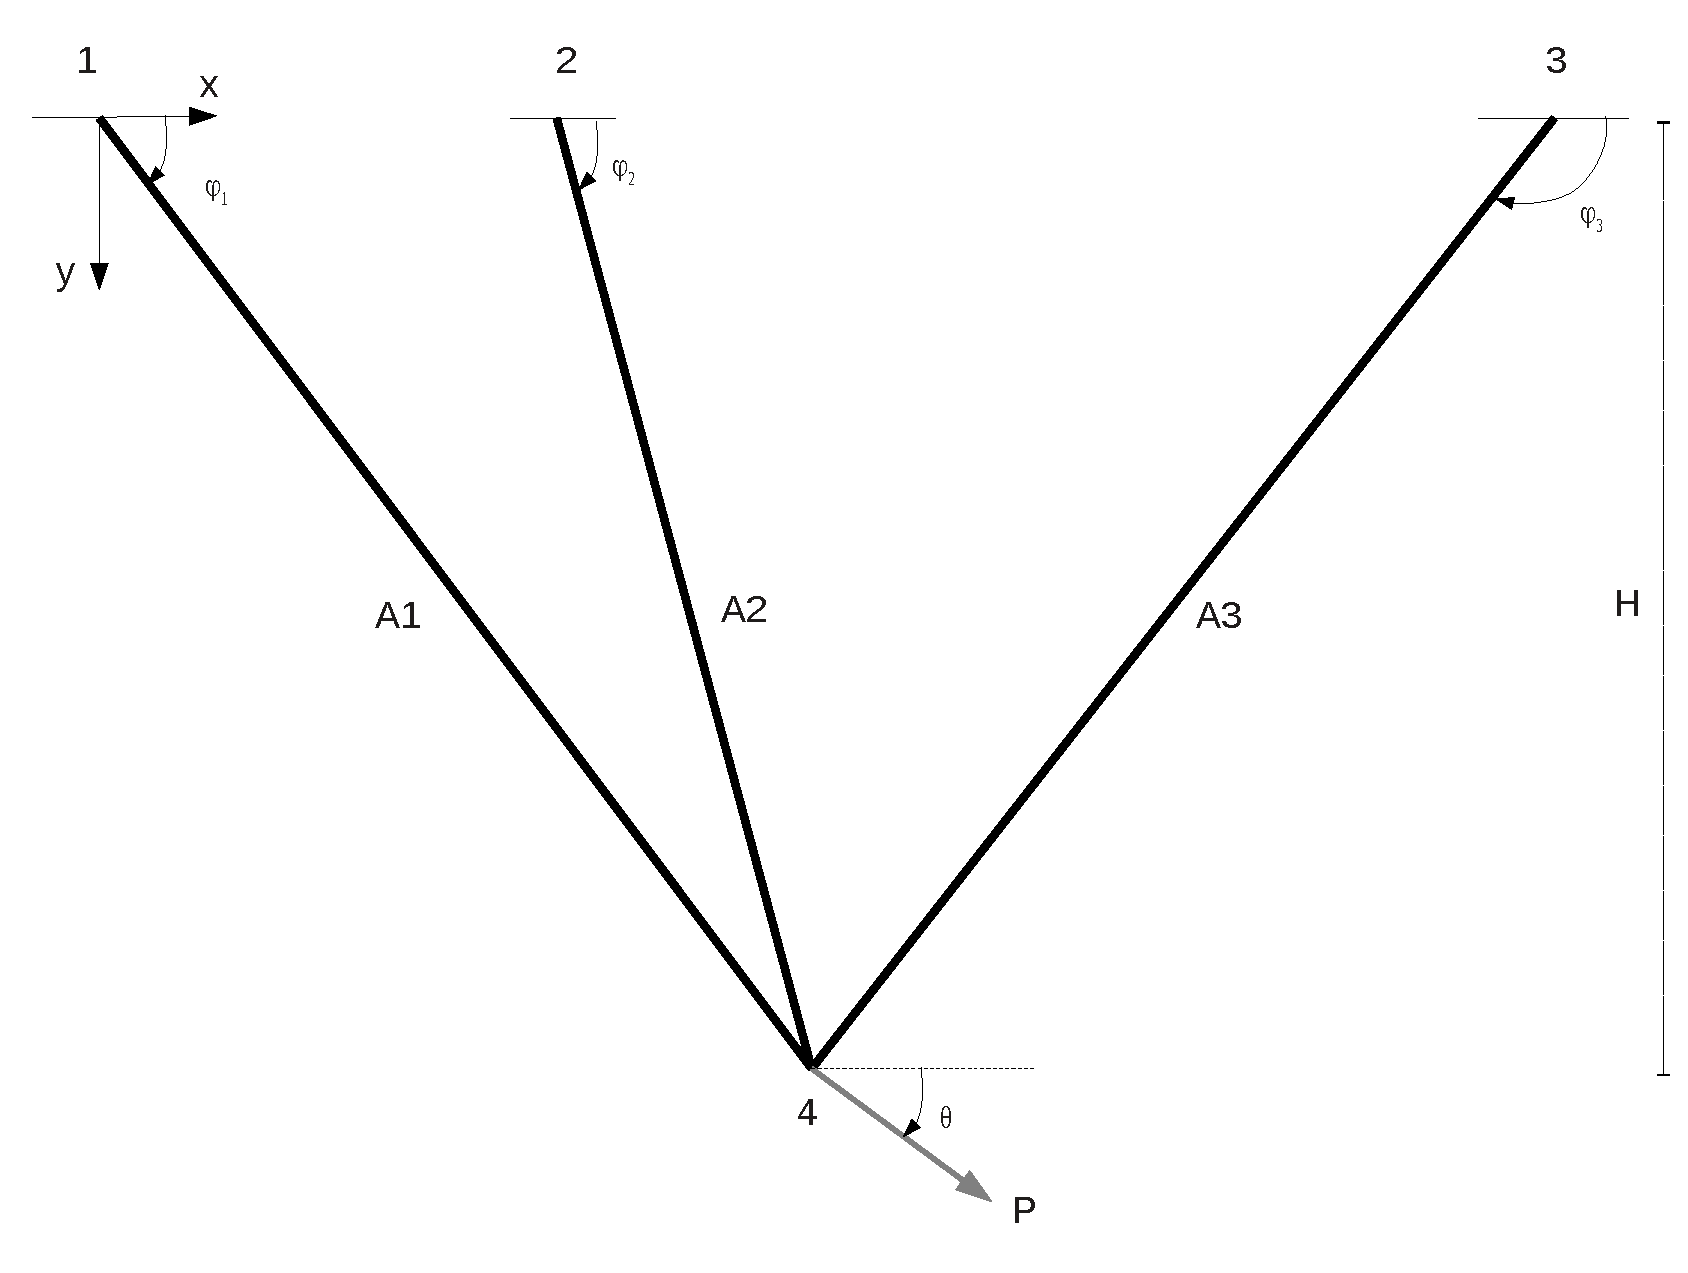
\includegraphics[width=1.0\textwidth]{3bargraphics.eps} 
  \end{minipage}
\caption{A schematic diagram of the three-bar truss structure.}
\label{fig:3bar}
\end{figure}
\subsection{Deterministic Problem}

 

The truss shown in Figure~\ref{fig:3bar} is subjected to a load inclined at an angle $\theta$ from the horizontal, which puts bars $1$ and $2$ under tension and bar $3$ under compression. The nodes are represented with numbers 1 through 4. The goal is to minimize the total weight ${\W}$ of the structure.
The mathematical formulation of the problem is given below in Eq~(\ref{eq:3bardet}).
\beq \label{eq:3bardet}
\begin{aligned}
& \underset{\d}{\text{minimize}} & & {\W} =\frac{A_1\gamma{H}}{\sin(\phi_1)}+\frac{A_2\gamma{H}}{\sin(\phi_2)}+\frac{A_3\gamma{H}}{\sin(\phi_3)}, \\
& \text{subject to} & & g_1 =\frac{\sigma_1}{\sigma_{1_{max}}} - 1 \leq 0,\\
& & & g_2 =\frac{\sigma_2}{\sigma_{2_{max}}} - 1 \leq 0,\\
& & & g_3 =\frac{\sigma_3}{\sigma_{3_{max}}} - 1 \leq 0,\\
& & & g_4 =-\frac{\sigma_1}{\sigma_{1_{max}}} - 1 \leq 0,\\
& & & g_5 =-\frac{\sigma_2}{\sigma_{2_{max}}} - 1\leq 0,\\
& & & g_6 =-\frac{\sigma_3}{\sigma_{3_{max}}} - 1\leq 0,\\
& & & g_7 =\frac{Q_{4x}}{Q_{4x_{max}}} - 1\leq 0,\\
& & & g_8 =\frac{Q_{4y}}{Q_{4y_{max}}} - 1\leq 0,\\
& \text{bounds} & & 0.25~in^2 \leq~A_1,~A_2,~ A_3~\leq 5.0~in^2, \\
&  & & 30^\circ \leq~\phi_1~\leq 60^\circ, \\
&  & & 60^\circ \leq~\phi_2~\leq 120^\circ, \\
&  & & 120^\circ \leq~\phi_3~\leq 150^\circ. \\
\end{aligned}
\eeq
% and $c \approx [P,~\theta,~E,~\gamma,~H]$.
The problem has a total of six design variables $\d=[A_1, A_2, A_3, \phi_1, \phi_2, \phi_3]$, \ie~ the areas ($A_1$, $A_2$ and $A_3$) and the orientations ($\phi_1$, $\phi_2$ and $\phi_3$) of the bars with respect to the horizontal. The structure has to be designed to withstand a total of 8 constraints $g_i({\d})$. It is to be noted that the constraints are normalized with respect to their allowable values (denoted with subscript $max$). The first three, the next three, and the last two constraints impose tensile stress, compressive stress and displacement requirements, respectively. The axial stresses and nodal displacements used in Eq.~(\ref{eq:3bardet}) are calculated using a finite element procedure described in Appendix~\ref{appendix:3bar}.
The other parameters used for this problem are listed in Table~\ref{tab:data_threebartruss}. 

\begin{table}[h!]
\caption{Design data for three-bar truss.}
\medskip
\centering 
\begin{tabular}{cccc}
\hline\hline
Quantity           & Description          & Value               & Unit\\
\hline\hline
P                  & Load                 & 30000                & $lb$ \\
$\theta$           & Loading angle        & $50$                 & $deg$\\
E                  & Young's modulus      & $10^7$               & $psi$ \\
$\gamma$           & Weight density       & 0.1                  & $lb/in^3$ \\
H                  & Reference length     & 10                   & $in$ \\
{}                  & (projection on $y-$axis)     & {}                   & {} \\
$\sigma_{1_{max}}$    & Allowable axial stress on bar 1  & 5000     & $psi$\\
$\sigma_{2_{max}}$    & Allowable axial stress on bar 2  & 10000    & $psi$\\
$\sigma_{3_{max}}$    & Allowable axial stress on bar 3  & 5000     & $psi$\\
$u_{4x_{max}}$        & Allowable x-displacement at 4    & 0.005    & $in$\\
$u_{4y_{max}}$        & Allowable y-displacement at 4    & 0.005     & $in$\\
$\epsilon_1$       & Constraint violation tolerance    & $10^{-3}$  & - \\
$\epsilon_2$       & Norm of design change $\|\Delta \d\|$            & $10^{-3}$  & - \\
\hline
\end{tabular}
\label{tab:data_threebartruss}
\end{table}

\subsection{Robust Optimization Problem}
The robust optimization problem involves minimizing the following objective function:
\beq \label{eq:3barrob}
\begin{aligned}
& \underset{\z,\n}{\text{minimize}}
& &  {\J}={\mu_{\W}}+{\sigma_{\W}^2}, \\
& \text{subject to}
& &  g_i^r={\mu_{g_i}+k\sigma_{g_i}}\le 0, \;~\mathrm{for}~i=1,\ldots,8,\\
%& & & g^r=g(\mus,\q,\z,\n) - k \sigma_g^*  \le 0.\\
%& \text{bounds}
%& & \d^\text{L} \le \d \le \d^\text{U}.
\end{aligned}
\eeq
i.e. the minimization of an equally weighted sum of the mean and variance of the weight subject to eight constraints.
The area design variables $A_i$ are assumed to have epistemic uncertainties with bounds $\tau_i= \pm 0.1 \,in^2$ and the orientations $\phi_i$ are assumed to have aleatory uncertainties with standard deviation $\sigma_i=1^\circ$. The input aleatory uncertainties are modeled as $\alpha^{(j)} \sim {\N}(\mu_{\phi_i},\sigma^2_{\phi_i})$ and the epistemic uncertainties are represented as an interval $\beta^{(j)} \in [A_i-\es_i,A_i+\es_i]$.
All other input parameters are kept fixed throughout the optimization.
\paragraph{Surrogate Models:}
The kriging surrogate model is built with seventy training points. The polynomial chaos surrogate is a fourth order polynomial with an oversampling factor of two which also requires seventy training points. The training points are chosen via the dynamic training point selection framework~\cite{Komahan2013c,Komahan2013a}.
Note that each training data $f^*$ comes from solving a BCO problem as discussed in section~\ref{bco}.

\subsection{Optimization Results}

\subsubsection{Deterministic and Robust Designs}

Table~\ref{tab:3baroptimum} compares the robust design optima with the deterministic optimum. From the optimum weights, it can be inferred that the deterministic design is the best in terms of lightness of the structure, but lacks robustness.
 A deterministic design with no assumed factor of safety is $15\%$ lighter than a highly robust design specified by $k=4$.
However, a deterministic design with a small factor of safety of 1.3 is $29\%$ heavier than a highly robust design specified by $k=4$. The designers can capitalize such a behavior for over-conservative designs that are in use today or the ones that need to be built in the future.
 A design corresponding to $k=0$ with a weight of $14.65\pm 0.24$ has  $50\%$ chances of violating the constraints and is not so robust compared to a design corresponding to $k=3$ with a weight of $16.54\pm 0.25$ that has less than one percent probability of violating the constraints. 
As the desired robustness specified with $k$ increases, an increase in the objective function value can be seen, meaning that robustness is obtained at the expense of additional weight to the structure.
The designer can carry out a trade-off study between the weight of the structure and the required robustness specified with $k$ or $P_k$.
It can be seen that the kriging and polynomial chaos based results agree very closely for all the tested cases.

\begin{table}[h!]
\caption{Optimization results for three-bar truss problem.}
\medskip
\centering 
\scalebox{0.75}{\begin{tabular}{c|cc|cccccc|ccc|c}
\hline\hline
Type  & k  & $P_k$ & $A_1$ & $A_2$ & $A_3$ & $\phi_1$ & $\phi_2$ & $\phi_3$ & $\mu_{\W}$ & ${\sigma_{\W}}$ & $C_v$ & No. of F/FG Evals. \\
{}  & {}  & ${}$ &  $in^2$ & $in^2$ & $in^2$ & $deg$ & $deg$ & $deg$ & $lb$ & $lb$ & {-} & $\&$ Iterations \\
\hline\hline
Initial design  & -  &    -   & 2.0 & 2.0 & 2.0 & 45.0 & 90.0 & 135.0 & 7.66   & - & - & {-} \\
\hline
Det $F_s=1.0$ & -  &    -   & 5.00 & 1.42 & 2.30 & 37.6 & 60.0 & 150.0  & 14.45 & - & - &  108/108-12  \\
Det $F_s=1.3$ & -  &    -   & 5.00 & 4.95 & 5.00 & 39.5 & 60.0 & 143.6  & 22.00 & - & - &  126/126-14  \\
\hline
Robust-KR  & 0  & 0.5000 & 5.00 & 1.45 & 2.37 & 37.7 & 60.0 & 150.0 & 14.65 & 0.24 & 0.0162 & 17559/17559-12 \\
Robust-PC  & 0  & 0.5000 & 5.00 & 1.45 & 2.37 & 37.7 & 60.0 & 150.0 & 14.65 & 0.24 & 0.0162 & 17615/17615-12 \\
\hline
Robust-KR  & 1  & 0.8413 & 5.00 & 1.66 & 2.66 & 37.5 & 60.0 & 149.3 & 15.41 & 0.24 & 0.0159 & 21963/21963-14 \\
Robust-PC  & 1  & 0.8413 & 5.00 & 1.66 & 2.66 & 37.5 & 60.0 & 149.3 & 15.41 & 0.24 & 0.0159 & 20555/20555-13 \\
\hline
Robust-KR  & 2  & 0.9772 & 5.00 & 1.84 & 2.92 & 37.5 & 60.0 & 148.6 & 16.02 & 0.25& 0.0155 & 23594/23594-13 \\
Robust-PC  & 2  & 0.9772 & 5.00 & 1.84 & 2.92 & 37.5 & 60.0 & 148.6 & 16.02 & 0.25& 0.0155 & 33555/33555-18 \\
\hline
Robust-KR  & 3  & 0.9986 & 5.00 & 1.99 & 3.15 & 37.5 & 60.0 & 148.2 & 16.54 & 0.25& 0.0153 & 20771/20771-12\\
Robust-PC  & 3  & 0.9986 & 5.00 & 1.99 & 3.15 & 37.5 & 60.0 & 148.2 & 16.54 & 0.25& 0.0153 & 17938/17938-12\\
\hline
Robust-KR  & 4  & 0.9999 & 5.00 & 2.13 & 3.36 & 37.6 & 60.0 & 147.9 & 17.00 & 0.26& 0.0151 & 31178/31178-17\\
Robust-PC  & 4  & 0.9999 & 5.00 & 2.13 & 3.36 & 37.6 & 60.0 & 147.9 & 17.00 & 0.26& 0.0151 & 19500/19500-12\\
\hline
\end{tabular}}
\label{tab:3baroptimum}
\end{table}
%\end{landscape}




It can also be noted that area $A_1$ is pushed to its upper limit for all designs, while the other two areas ($A_2$ and $A_3$) and orientations generally govern the robustness of the structure.

Since the standard deviation is always associated with a mean it is advantageous to use a dimensionless number, the coefficient of variation $C_v$ (also known as relative standard deviation or relative amount of uncertainty)~\cite{Arora2007} 
that measures the extent of variability in relation to the mean of the output. It can be used as a metric of comparison with different data sets or designs that involve different units, or different assumed input mean and standard deviations. A decrease in the coefficient of variation can be observed across the robust designs.
 
\subsubsection{Simulation Requirements}
\begin{figure}[h!]
  \centering  
  \begin{minipage}[b]{0.8\linewidth}
    \includegraphics[width=1.0\textwidth]{3bariterhist.eps} 
  \end{minipage}
  \caption[Optimization history for three-bar truss design problem.]{Change in the objective function with the number of optimizer iterations.}
  \label{3bariterhist}
\end{figure}
Table~\ref{tab:3baroptimum} also presents the number of exact function and gradient evaluations needed to reach the final design. Here, each constraint evaluation is counted towards the total number of simulations. 
The box-constrained optimization takes $2-3$ exact function and gradient evaluations for this test case. On average, the kriging and polynomial chaos took roughly the same number of function and gradient evaluations to reach the optimum.
Figure~\ref{3bariterhist} plots the change in the objective function with the number of optimizer iterations. 
%In many applications constraint values are available out of a single finite-element analysis. Considering this, the robust optimization for this problem takes approximately $2500$ function and gradient evaluations in total for a specified robust design.



%PDF OF OUTPUT FUNCTION

\subsubsection{Constraint Status}
\begin{table}[h!]
\caption{Constraint status for three-bar truss problem.}
\medskip
\centering 
\scalebox{0.68}{\begin{tabular}{c|c|cccccccc}
\hline\hline
Type           & k  & ${g_1^r}$  & ${g_2^r}$   & ${g_3^r}$   & ${g_4^r}$   & ${g_5^r}$   &  ${g_6^r}$  &${g_7^r}$    & ${g_8^r}$  \\ 
\hline\hline
Initial design & -  & $0.12\cdot 10^{1}$ & $-0.43\cdot 10^{0}$ & $-0.21\cdot 10^{1}$ & $-0.32\cdot 10^{1}$ &  $-0.16\cdot 10^{1}$ &  $0.69\cdot 10^{-1}$ &  $0.14\cdot 10^{0}$  &  $0.23\cdot 10^{1}$ \\
\hline
Det $F_s=1.0$ & -  &  $-0.14\cdot 10^{0}$ & $-0.41\cdot 10^{0}$ & $-0.12\cdot 10^{1}$ & $-0.19\cdot 10^{1}$ &  $-0.16\cdot 10^{1}$ &  $0.82\cdot 10^{0}$ &  $-0.48\cdot 10^{-8}$  &  $-0.17\cdot 10^{-8}$ \\
Det $F_s=1.3$ & -  &  $-0.29\cdot 10^{0}$ & $-0.58\cdot 10^{0}$ & $-0.13\cdot 10^{1}$ & $-0.17\cdot 10^{1}$ &  $-0.14\cdot 10^{1}$ &  $0.71\cdot 10^{0}$ &  $-0.46\cdot 10^{0}$  &  $-0.34\cdot 10^{-7}$ \\
\hline
Robust-KR  & 0   &  $-0.15\cdot 10^{0}$ & $-0.41\cdot 10^{0}$ & $-0.12\cdot 10^{1}$ & $-0.18\cdot 10^{1}$ &  $-0.16\cdot 10^{1}$ &  $-0.82\cdot 10^{0}$ &  $-0.56\cdot 10^{-6}$  &  $-0.87\cdot 10^{-5}$ \\
Robust-PC  & 0   &  $-0.15\cdot 10^{0}$ & $-0.41\cdot 10^{0}$ & $-0.12\cdot 10^{1}$ & $-0.18\cdot 10^{1}$ &  $-0.16\cdot 10^{1}$ &  $-0.82\cdot 10^{0}$ &  $-0.84\cdot 10^{-5}$  &  $-0.78\cdot 10^{-5}$ \\
\hline
Robust-KR  & 1   &  $-0.17\cdot 10^{0}$ & $-0.42\cdot 10^{0}$ & $-0.11\cdot 10^{1}$ & $-0.18\cdot 10^{1}$ &  $-0.15\cdot 10^{1}$ &  $-0.79\cdot 10^{0}$ &  $0.90\cdot 10^{-4}$  &  $0.49\cdot 10^{-4}$ \\
Robust-PC  & 1  &  $-0.17\cdot 10^{0}$ & $-0.42\cdot 10^{0}$ & $-0.11\cdot 10^{1}$ & $-0.18\cdot 10^{1}$ &  $-0.15\cdot 10^{1}$ &  $-0.79\cdot 10^{0}$ &  $-0.12\cdot 10^{-4}$  &  $0.38\cdot 10^{-4}$ \\
\hline
Robust-KR  & 2  & $-0.19\cdot 10^{0}$ & $-0.43\cdot 10^{0}$ & $-0.11\cdot 10^{1}$ & $-0.18\cdot 10^{1}$ &  $-0.15\cdot 10^{1}$ &  $0.77\cdot 10^{0}$ &  $-0.73\cdot 10^{-4}$  &  $0.13\cdot 10^{-3}$ \\
Robust-PC  & 2  & $-0.19\cdot 10^{0}$ & $-0.43\cdot 10^{0}$ & $-0.11\cdot 10^{1}$ & $-0.18\cdot 10^{1}$ &  $-0.15\cdot 10^{1}$ &  $0.77\cdot 10^{0}$ &  $-0.16\cdot 10^{-4}$  &  $-0.12\cdot 10^{-3}$ \\
\hline
Robust-KR  & 3  &  $-0.20\cdot 10^{0}$ & $-0.43\cdot 10^{0}$ & $-0.11\cdot 10^{1}$ & $-0.17\cdot 10^{1}$ &  $-0.15\cdot 10^{1}$ &  $0.76\cdot 10^{0}$ &  $0.28\cdot 10^{-3}$  &  $-0.12\cdot 10^{-3}$ \\
Robust-PC  & 3  &  $-0.20\cdot 10^{0}$ & $-0.43\cdot 10^{0}$ & $-0.11\cdot 10^{1}$ & $-0.17\cdot 10^{1}$ &  $-0.15\cdot 10^{1}$ &  $0.76\cdot 10^{0}$ &  $0.16\cdot 10^{-3}$  &  $-0.76\cdot 10^{-4}$ \\
\hline
Robust-KR  & 4  &  $-0.21\cdot 10^{0}$ & $-0.43\cdot 10^{0}$ & $-0.11\cdot 10^{1}$ & $-0.17\cdot 10^{1}$ &  $-0.14\cdot 10^{1}$ &  $-0.74\cdot 10^{-3}$ &  $0.90\cdot 10^{-4}$  &  $0.20\cdot 10^{-3}$ \\
Robust-PC  & 4  &  $-0.21\cdot 10^{0}$ & $-0.43\cdot 10^{0}$ & $-0.11\cdot 10^{1}$ & $-0.17\cdot 10^{1}$ &  $-0.14\cdot 10^{1}$ &  $-0.74\cdot 10^{-3}$ &  $0.75\cdot 10^{-3}$  &  $-0.36\cdot 10^{-3}$ \\
\hline
\end{tabular}}
\label{tab:3barconstat}
\end{table}
%\end{landscape}

Table~\ref{tab:3barconstat} displays the status of all eight constraints at the initial design, deterministic optimum, and robust optimum. 
Here, a positive value for $g$ represents a constraint-violation, whereas a negative value means that the constraint is satisfied.
It can be inferred that constraints 1, 7 and 8 are the ones that significantly affect the design throughout the optimization (tight or $\epsilon$-active constraints). 
The kriging and polynomial chaos based values are a little different for these tight constraints, yet within the specified tolerance to ensure that the constraints are not violated.
All other constraints are inactive and both the surrogate models provide same values to these constraints. 


\subsubsection{Output PDF and CDF}
Figures~\ref{3barPDF} and \ref{3barCDF} show the probability density function (PDF) and cumulative distribution function (CDF) of the objective function (weight) as well as the constraints (normalized) at their optimum designs.
As the desired robustness specified with $k$ increases, an increase in the objective function value by means of a shift to the right can be seen.
The robust optimization problem formulation serves to move the constraint values $k$ standard deviations away from a potential violation which is evident from the PDF and CDF of the constraints. It can be seen that a design corresponding to $k=4$ has less than $1\%$ chances of constraint violation, whereas $k=0$ features $50\%$ chances of constraint violation due to the effect of input uncertainties.
\begin{figure}[H]
  \centering  
  \begin{minipage}[b]{0.32\linewidth}
    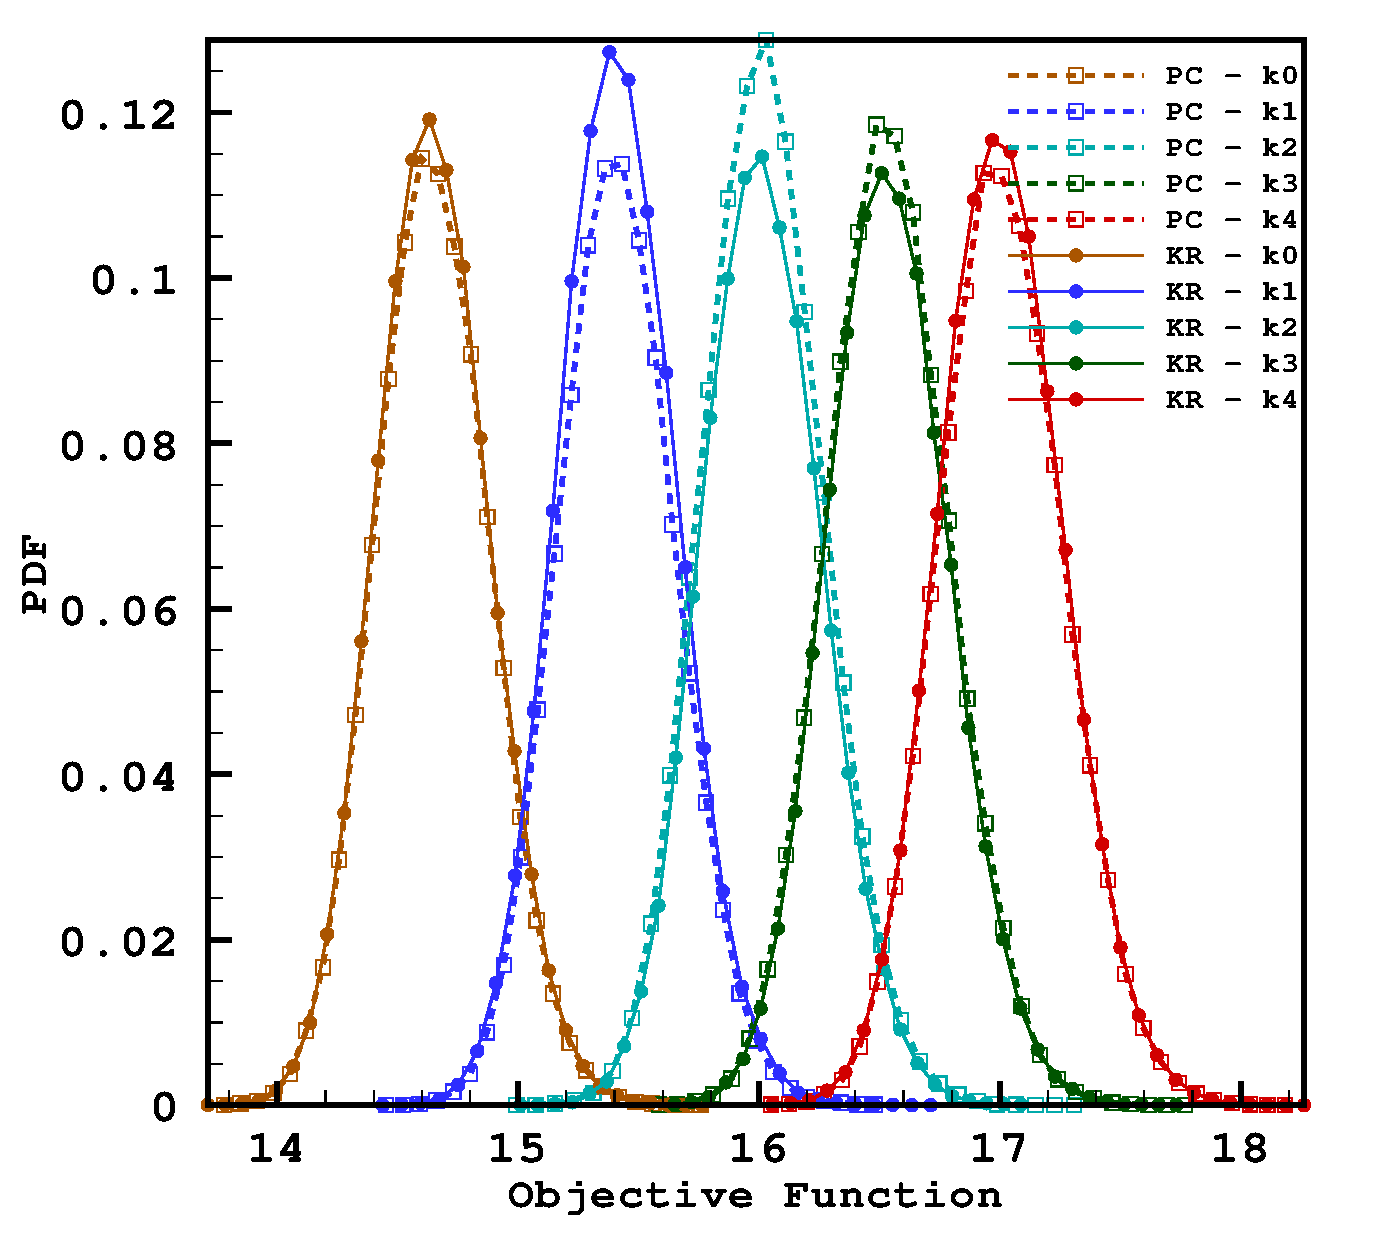
\includegraphics[width=1.0\textwidth]{3barpdfallcon0.eps} \subcaption{Cost function}
    \label{con0pdf}
  \end{minipage}
  \begin{minipage}[b]{0.32\linewidth}
    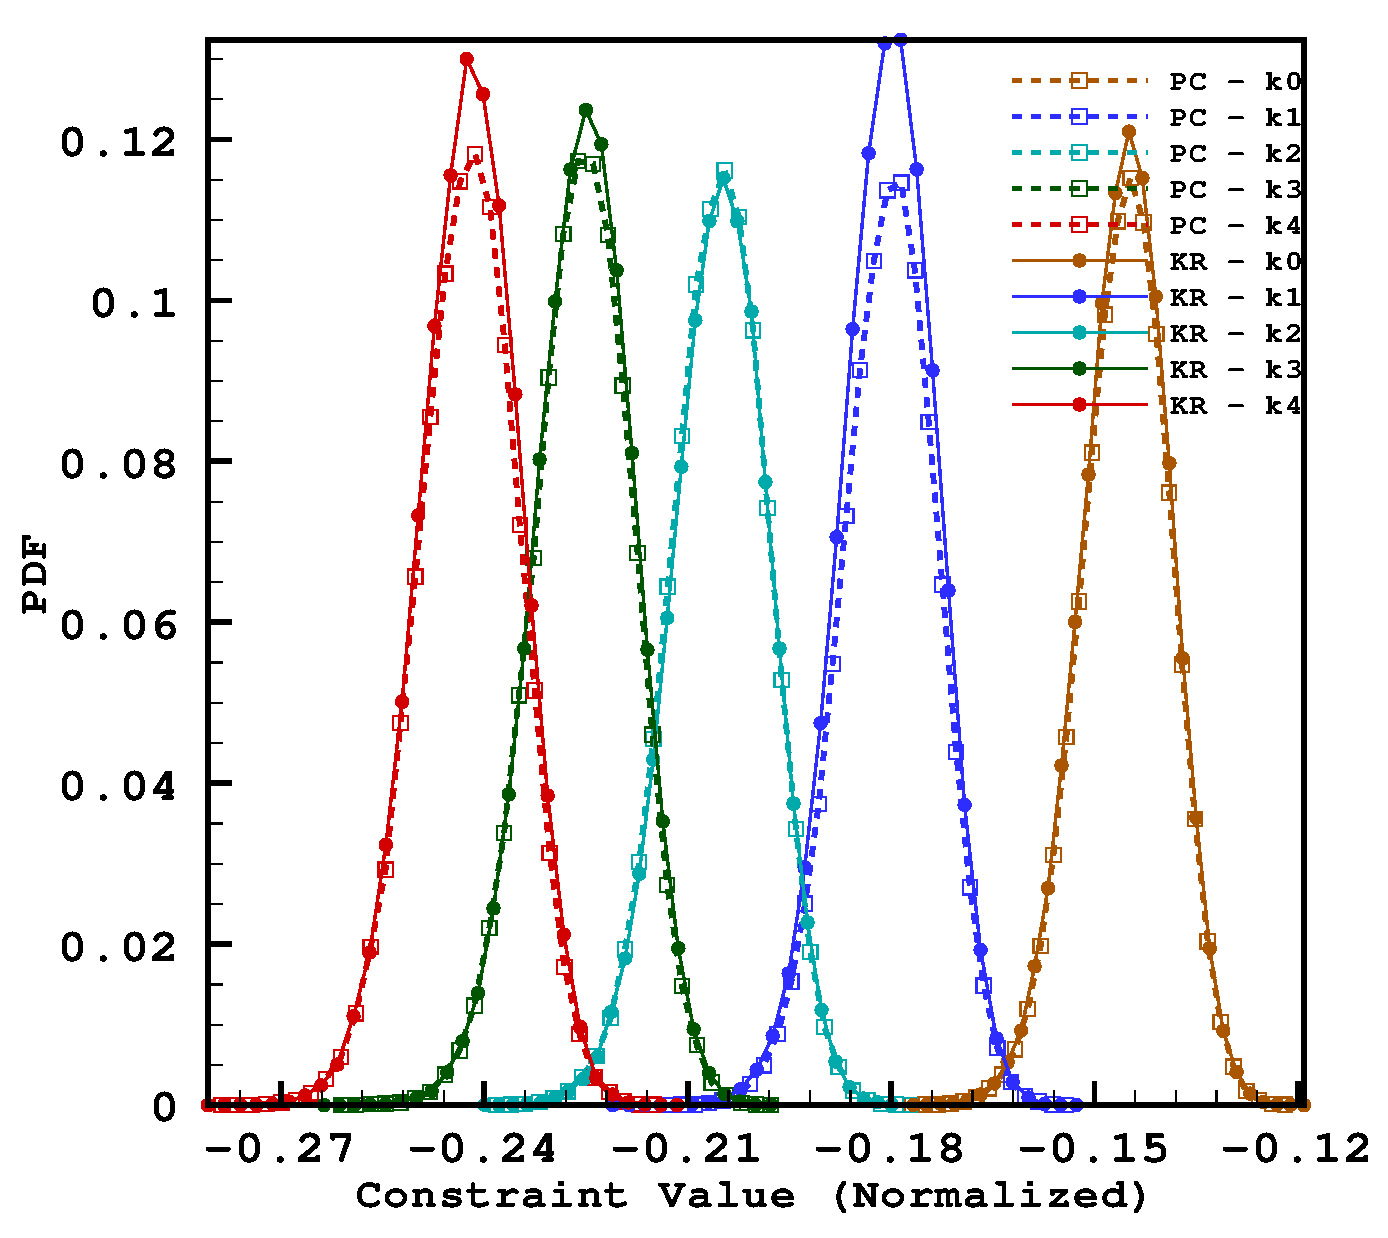
\includegraphics[width=1.0\textwidth]{3barpdfallcon1.eps} \subcaption{Constraint 1}
    \label{con1pdf}
  \end{minipage}
  \begin{minipage}[b]{0.32\linewidth}
    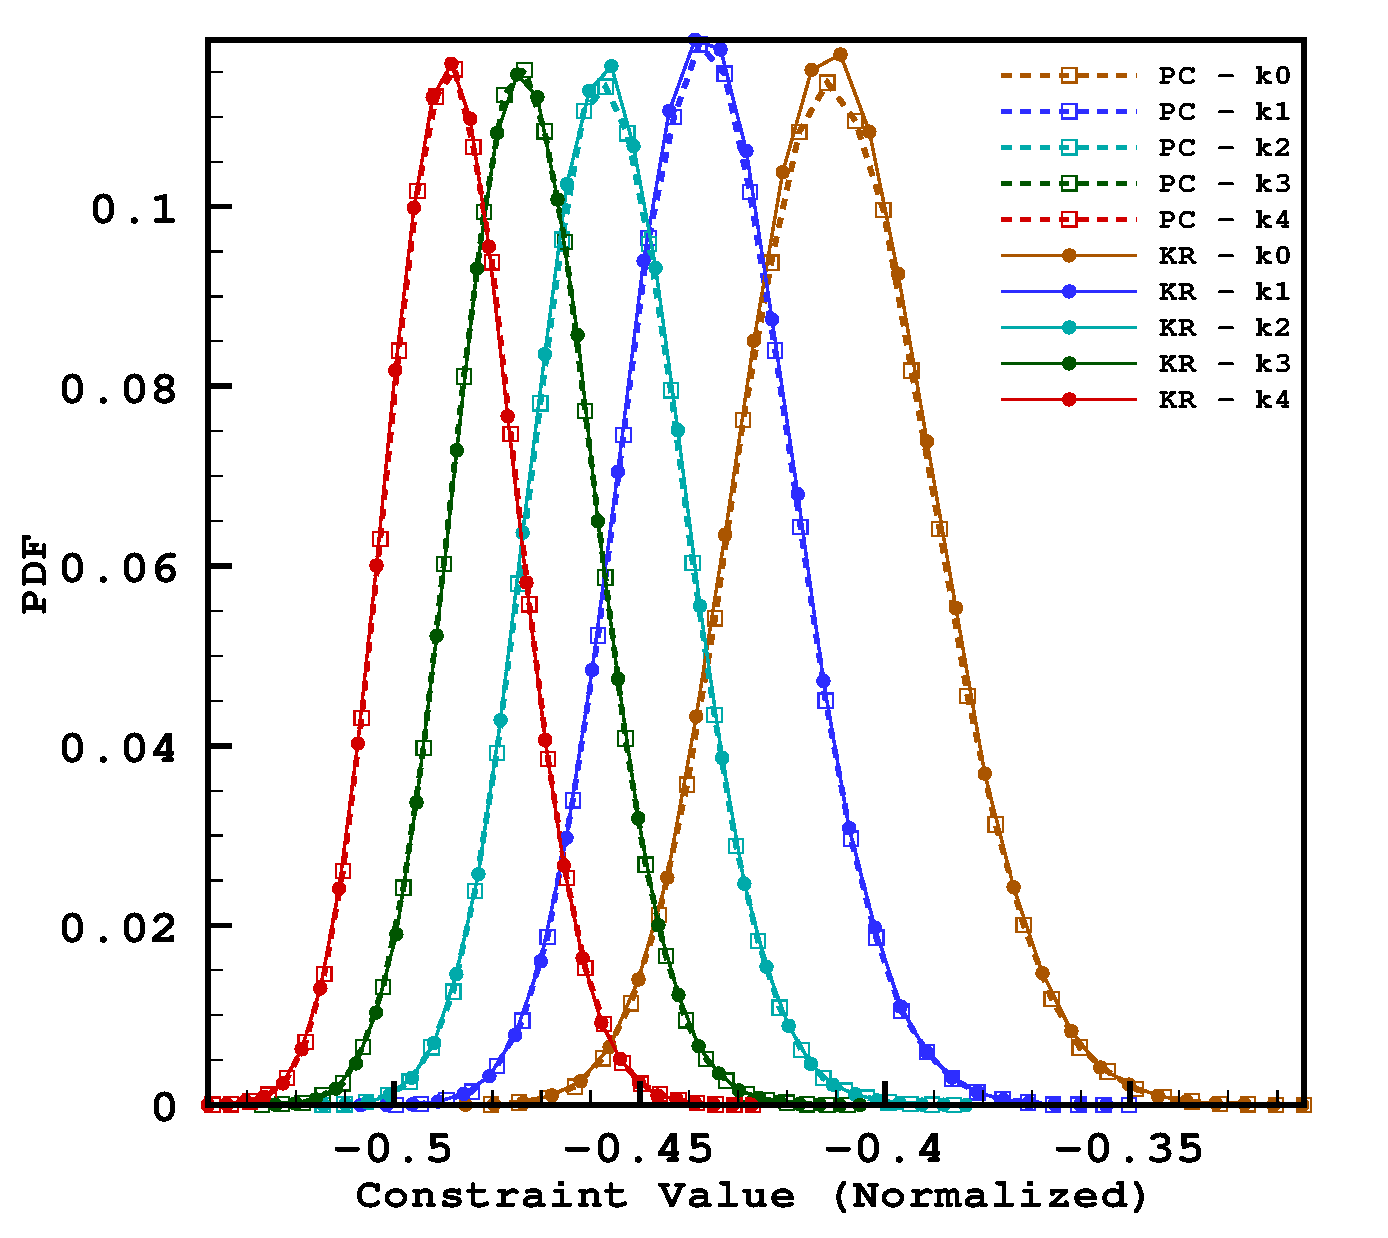
\includegraphics[width=1.0\textwidth]{3barpdfallcon2.eps} \subcaption{Constraint 2}
    \label{con2pdf}
  \end{minipage}
  \begin{minipage}[b]{0.32\linewidth}
    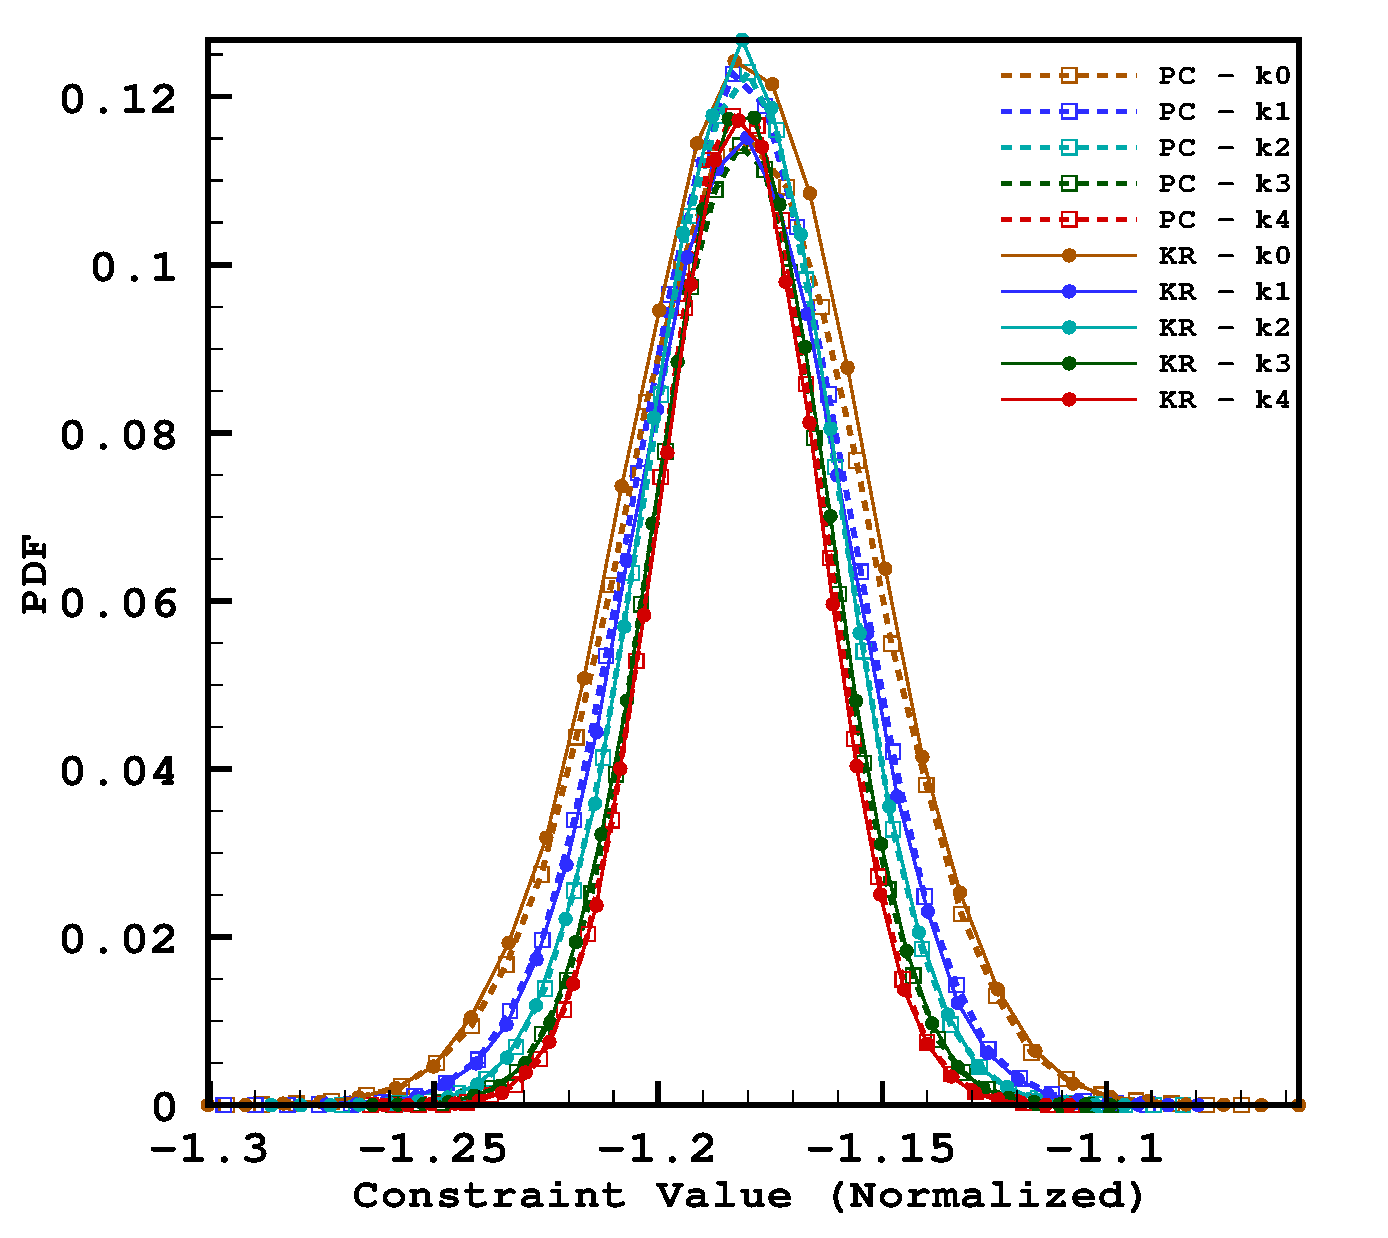
\includegraphics[width=1.0\textwidth]{3barpdfallcon3.eps} \subcaption{Constraint 3}
    \label{con3pdf}
  \end{minipage}
  \begin{minipage}[b]{0.32\linewidth}
    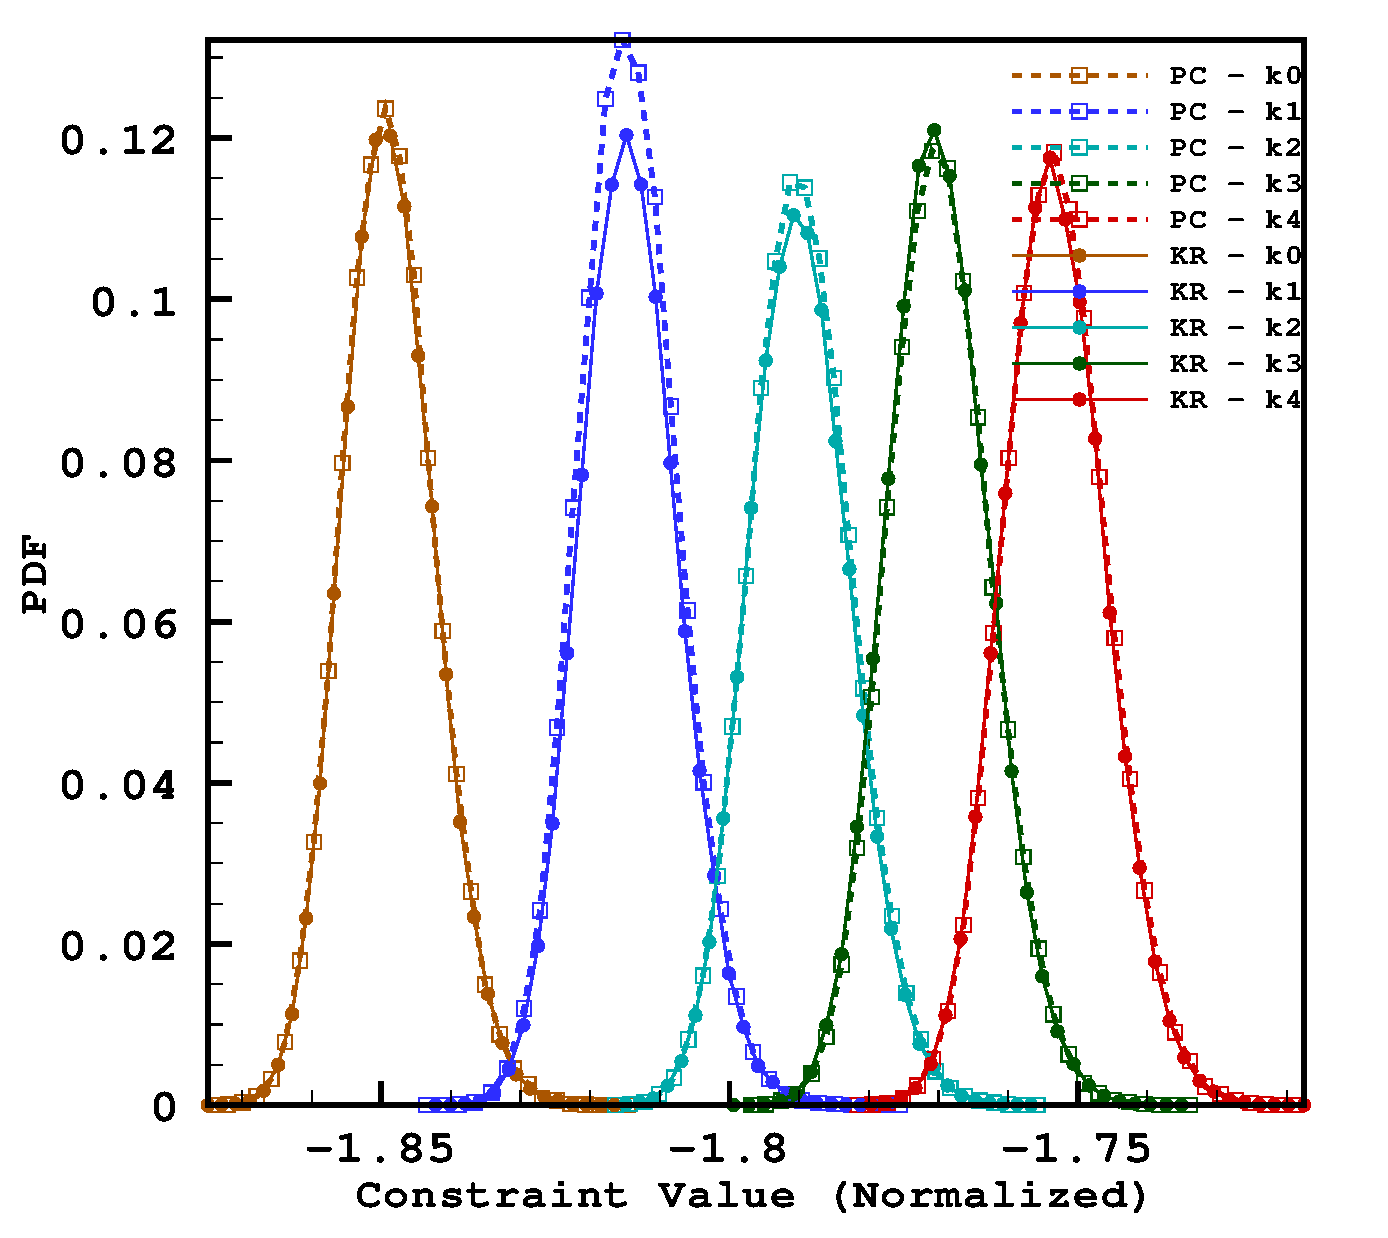
\includegraphics[width=1.0\textwidth]{3barpdfallcon4.eps} \subcaption{Constraint 4}
    \label{con4pdf}
  \end{minipage}
  \begin{minipage}[b]{0.32\linewidth}
    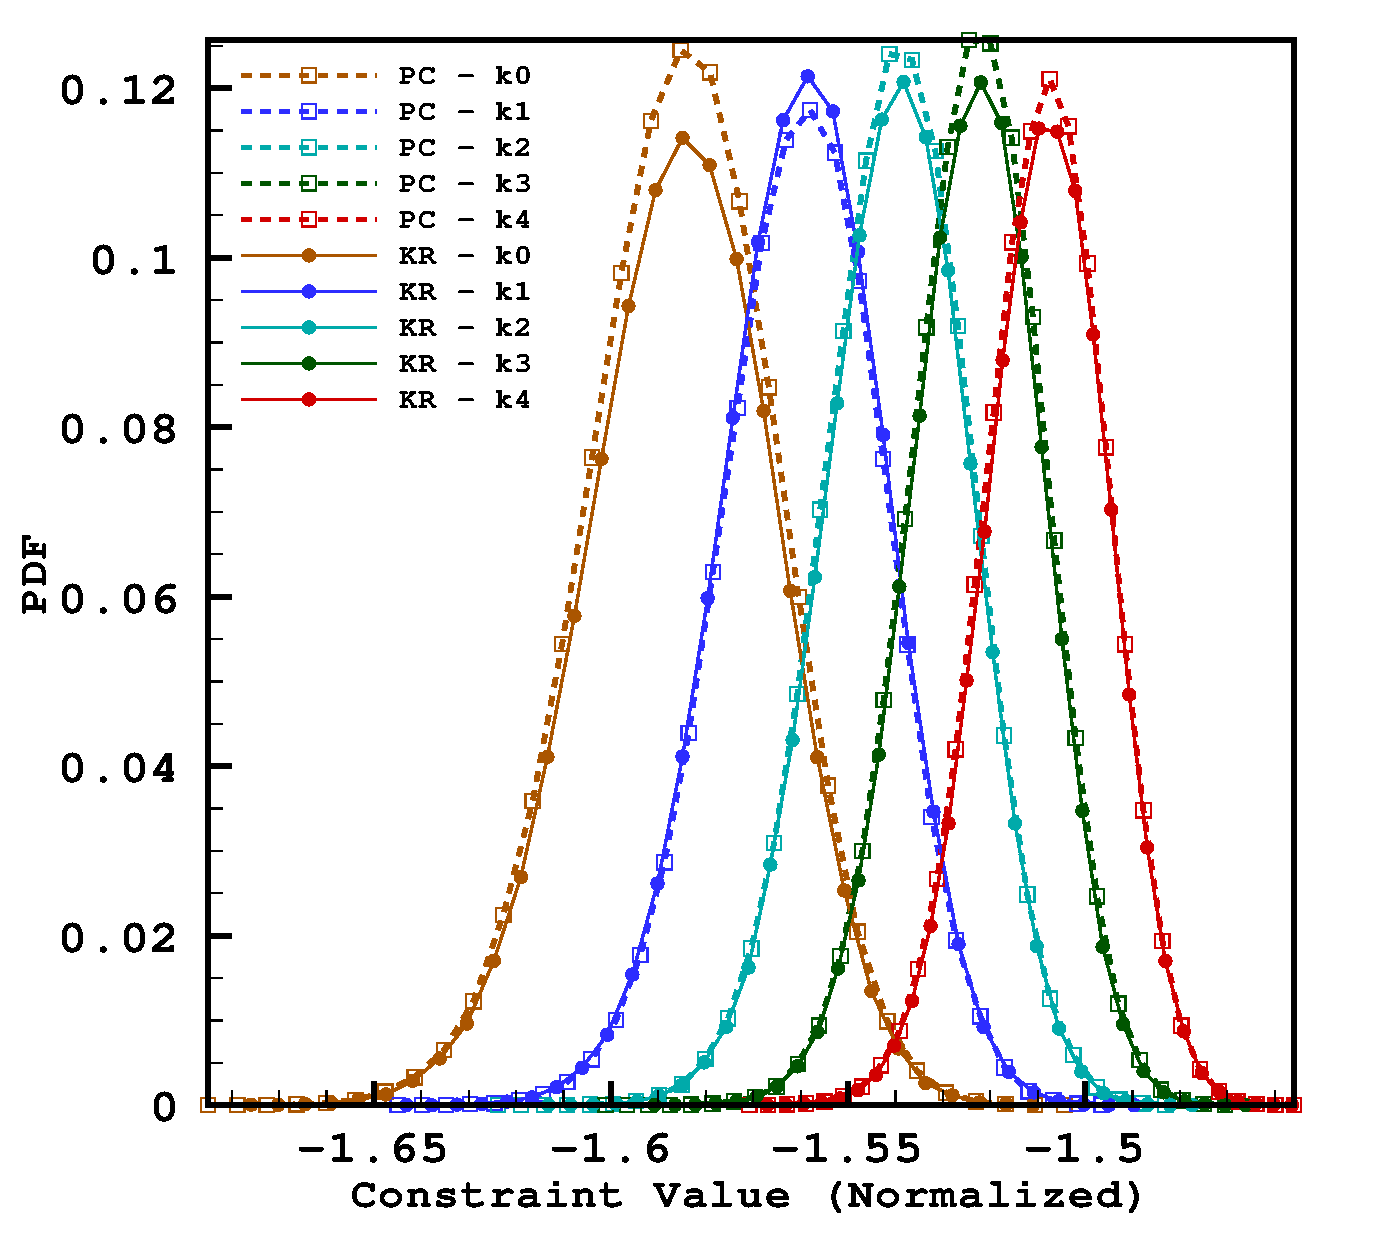
\includegraphics[width=1.0\textwidth]{3barpdfallcon5.eps} \subcaption{Constraint 5}
    \label{con5pdf}
  \end{minipage}
  \begin{minipage}[b]{0.32\linewidth}
    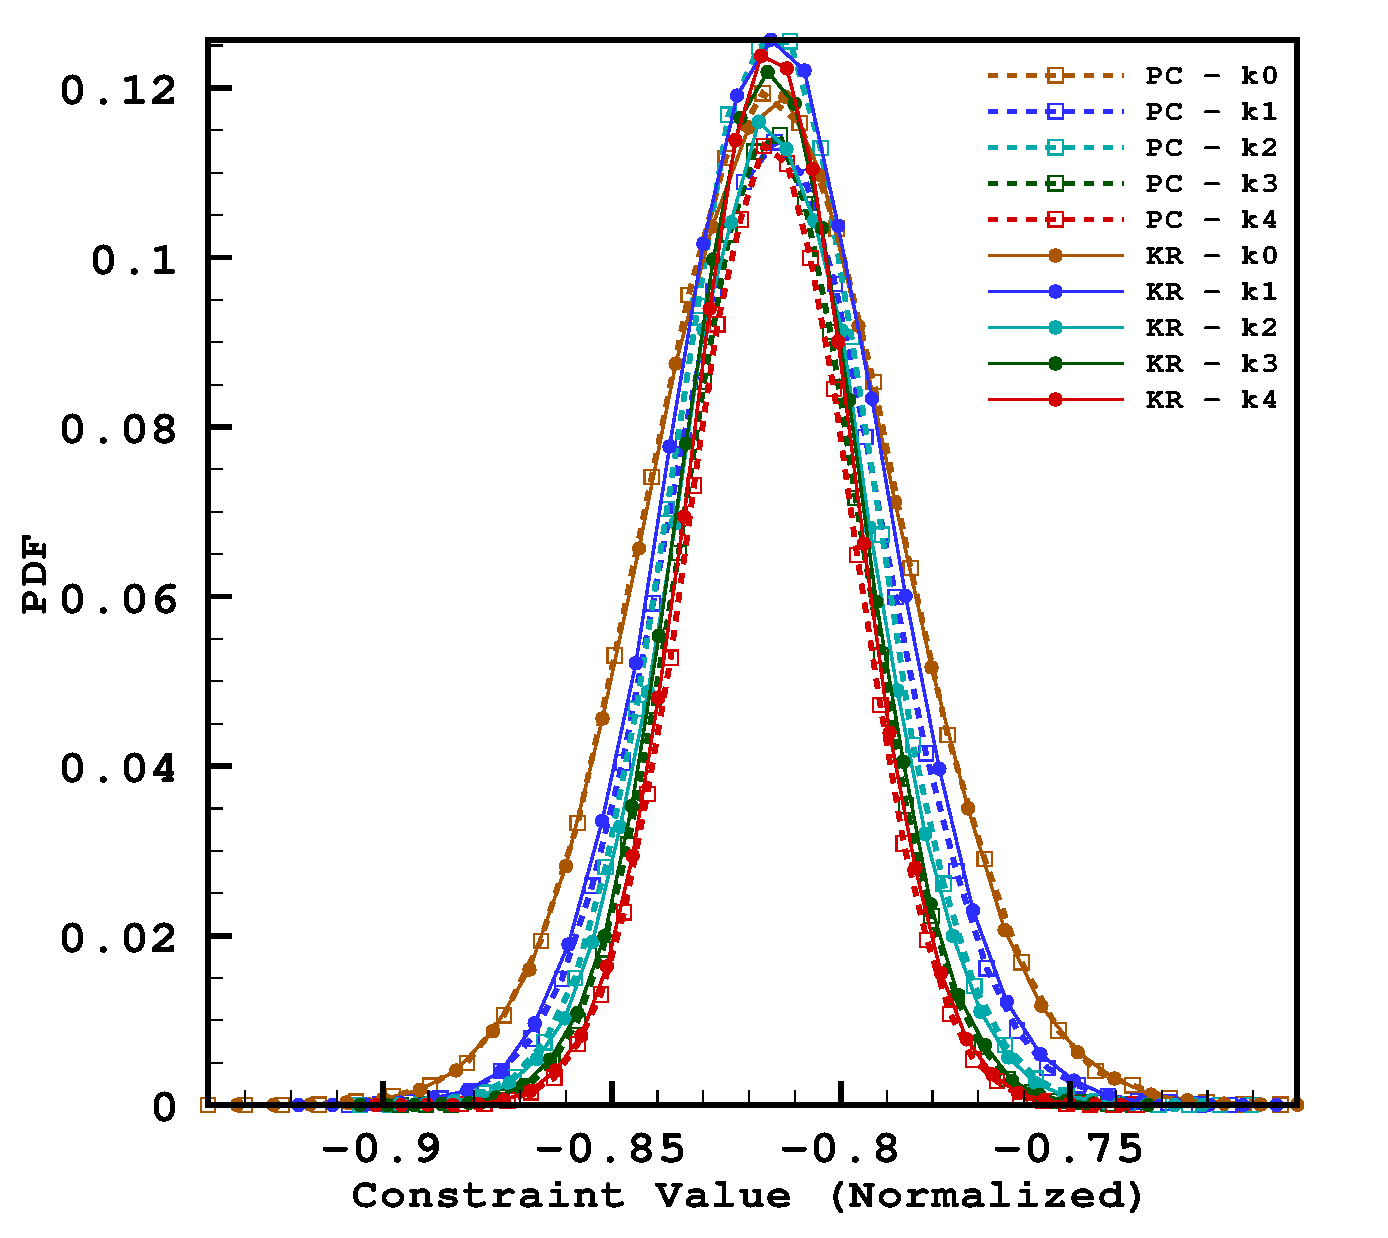
\includegraphics[width=1.0\textwidth]{3barpdfallcon6.eps} \subcaption{Constraint 6}
    \label{con6pdf}
  \end{minipage}
  \begin{minipage}[b]{0.32\linewidth}
    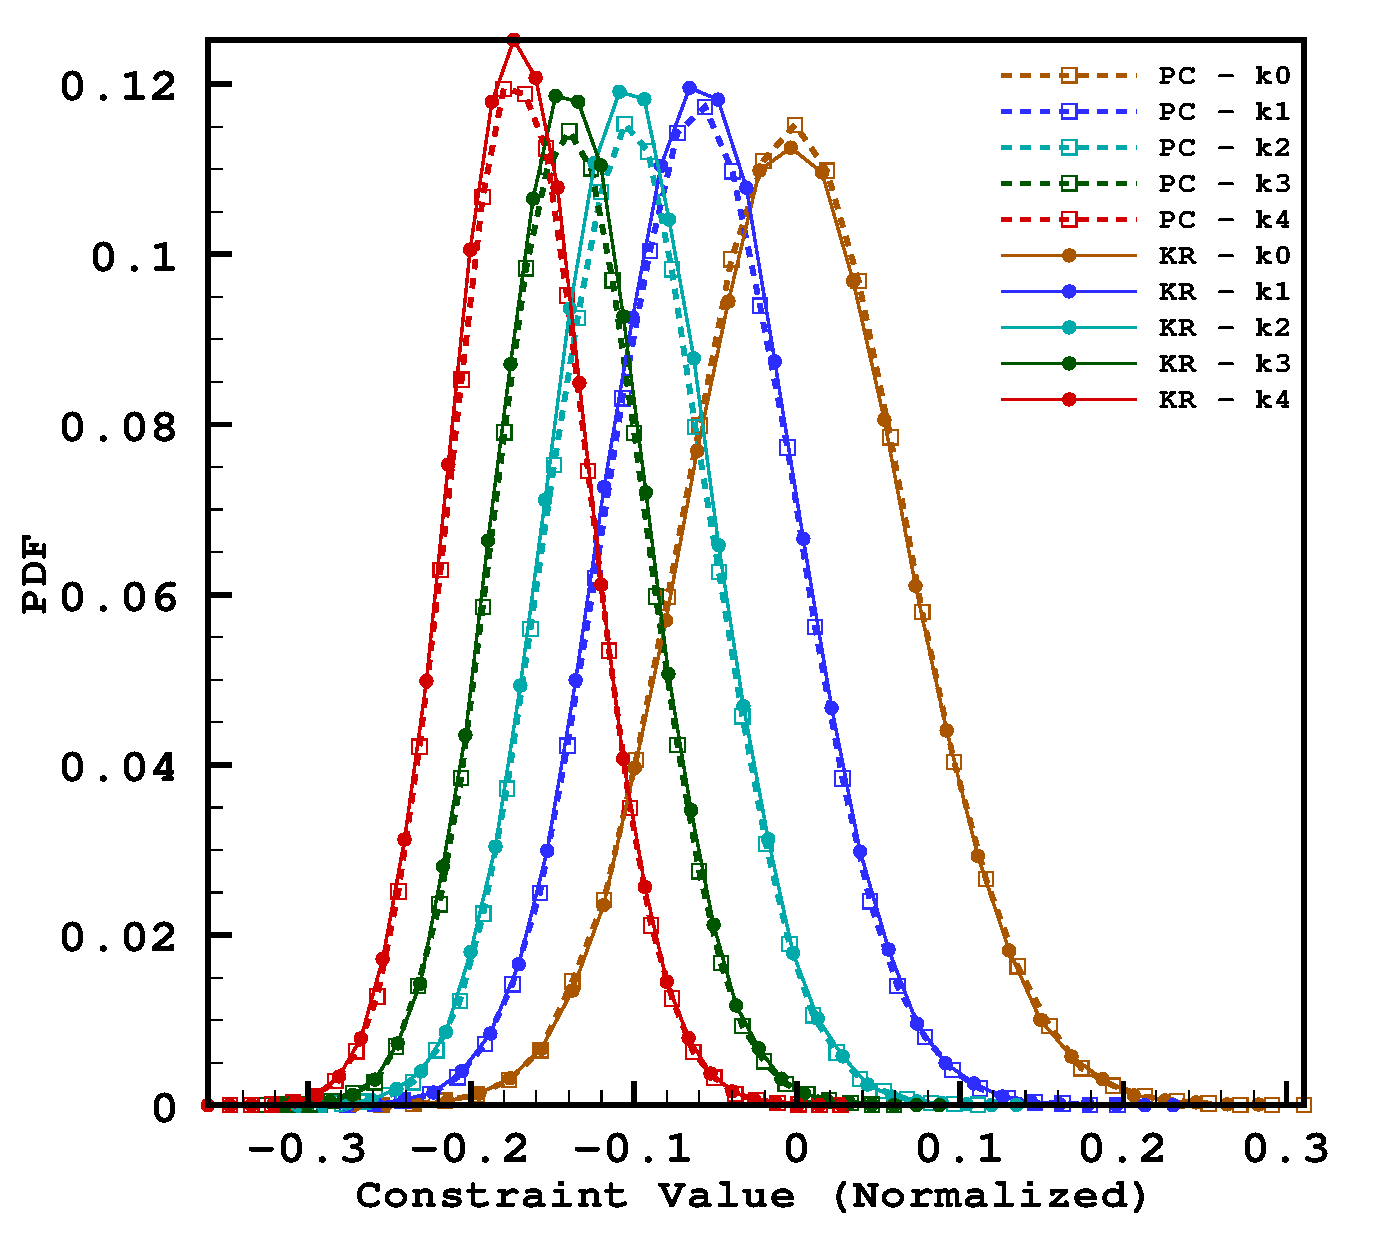
\includegraphics[width=1.0\textwidth]{3barpdfallcon7.eps} \subcaption{Constraint 7}
    \label{con7pdf}
  \end{minipage}
  \begin{minipage}[b]{0.32\linewidth}
    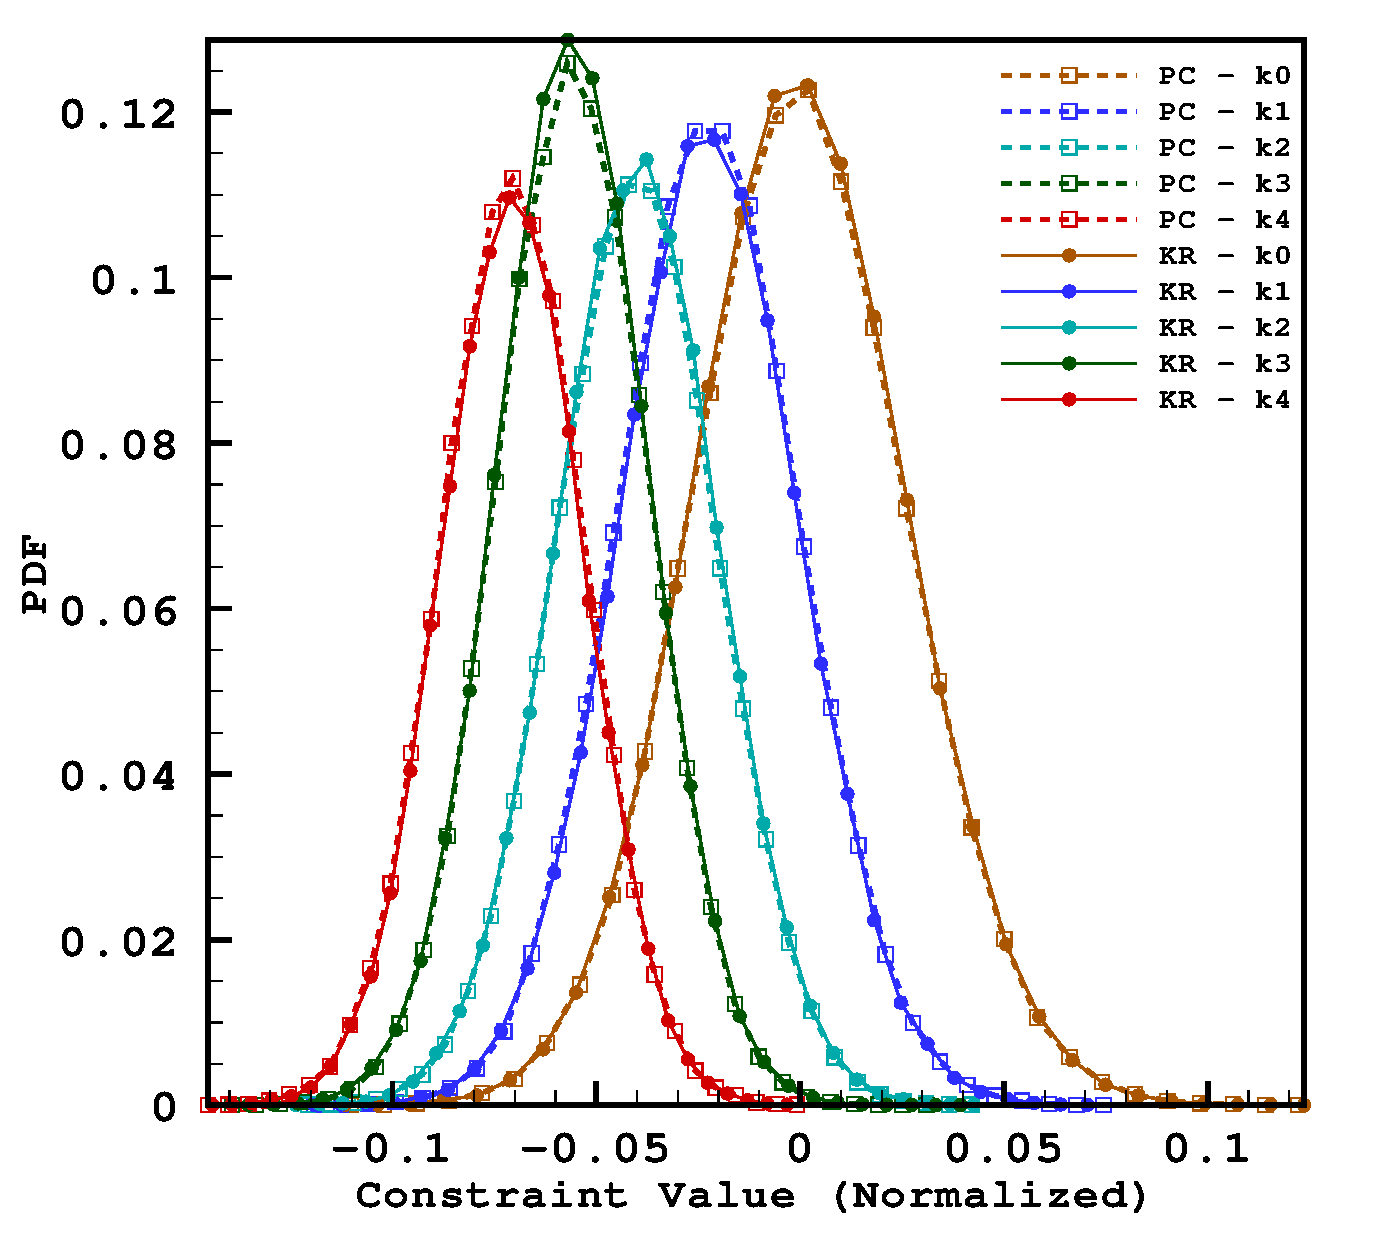
\includegraphics[width=1.0\textwidth]{3barpdfallcon8.eps} \subcaption{Constraint 8}
    \label{con8pdf}
  \end{minipage}
  \caption[Probability density functions for three-bar truss design problem.]{Probability density function of objective and constraint functions at robust optimum designs.}
  \label{3barPDF}
\end{figure}
 It can also be seen that the spread of values is reduced as the robustness increases (compare PDFs of $k=0$ and $k=4$ cases), which shows that the design is less sensitive to uncertainties/variations in the input.
 Overall both surrogate models produce comparable distributions apart from occasional differences. 


\begin{figure}[H]
  \centering  
  \begin{minipage}[b]{0.32\linewidth}
    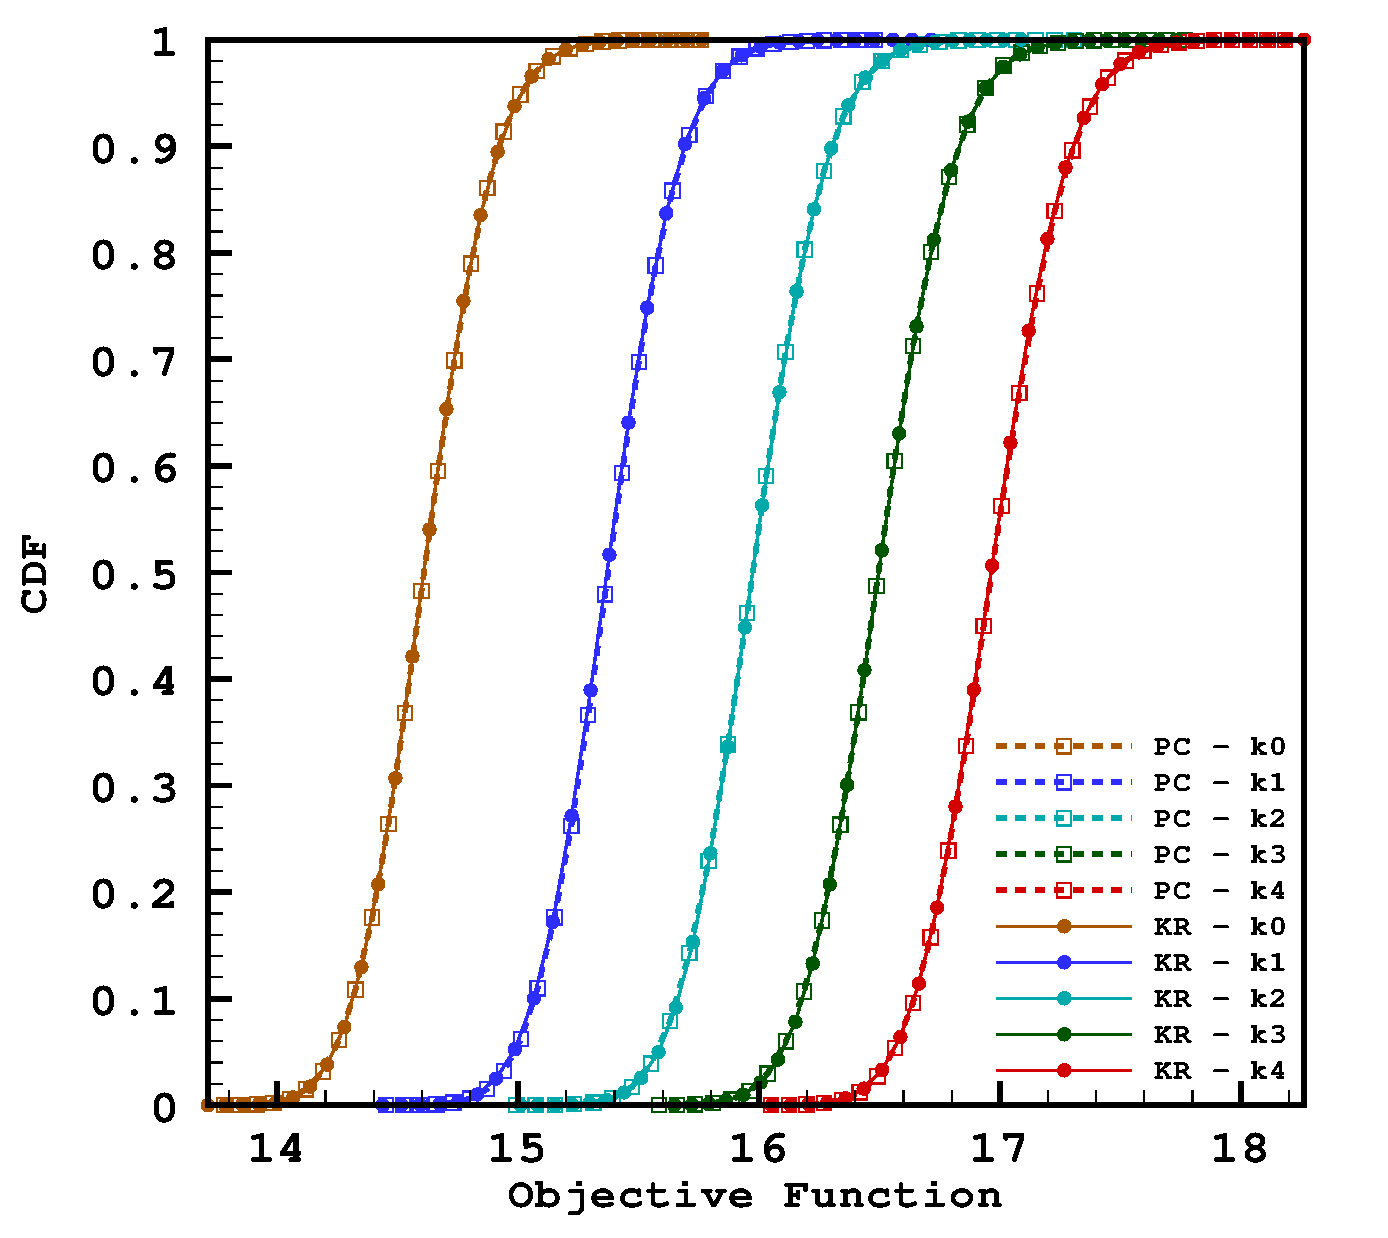
\includegraphics[width=1.0\textwidth]{3barcdfallcon0.eps} \subcaption{Cost function}
    \label{con0cdf}
  \end{minipage}
  \begin{minipage}[b]{0.32\linewidth}
    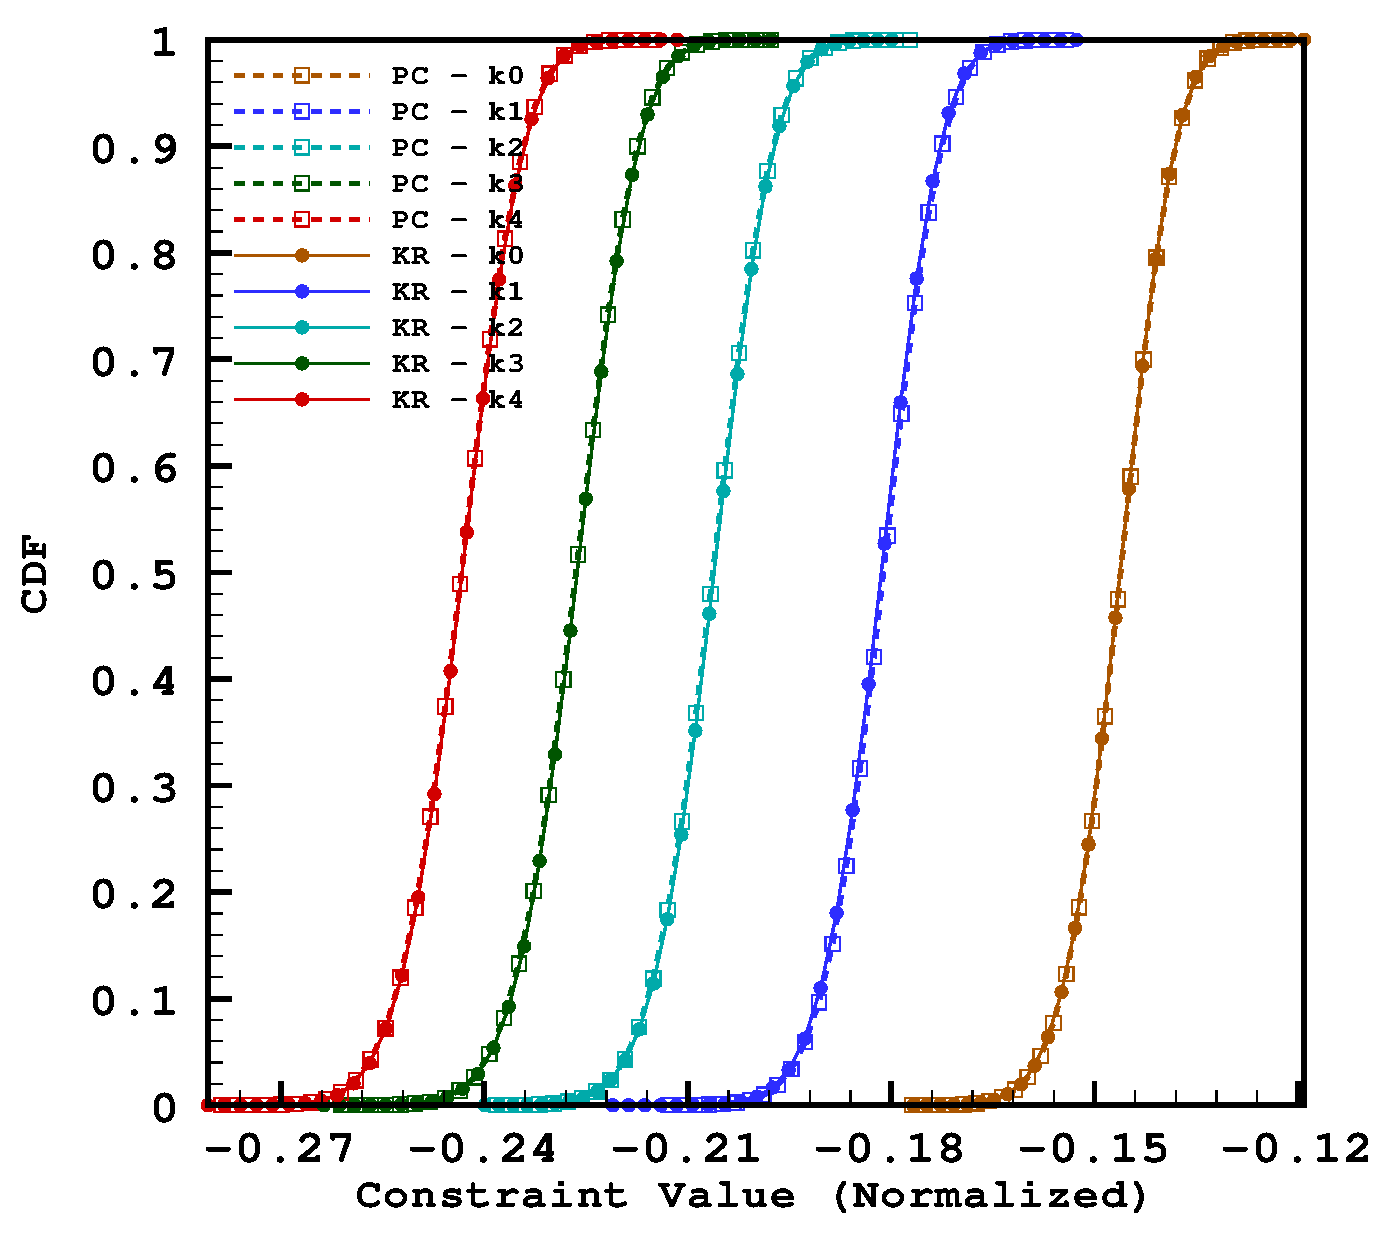
\includegraphics[width=1.0\textwidth]{3barcdfallcon1.eps} \subcaption{Constraint 1}
    \label{con1cdf}
  \end{minipage}
  \begin{minipage}[b]{0.32\linewidth}
    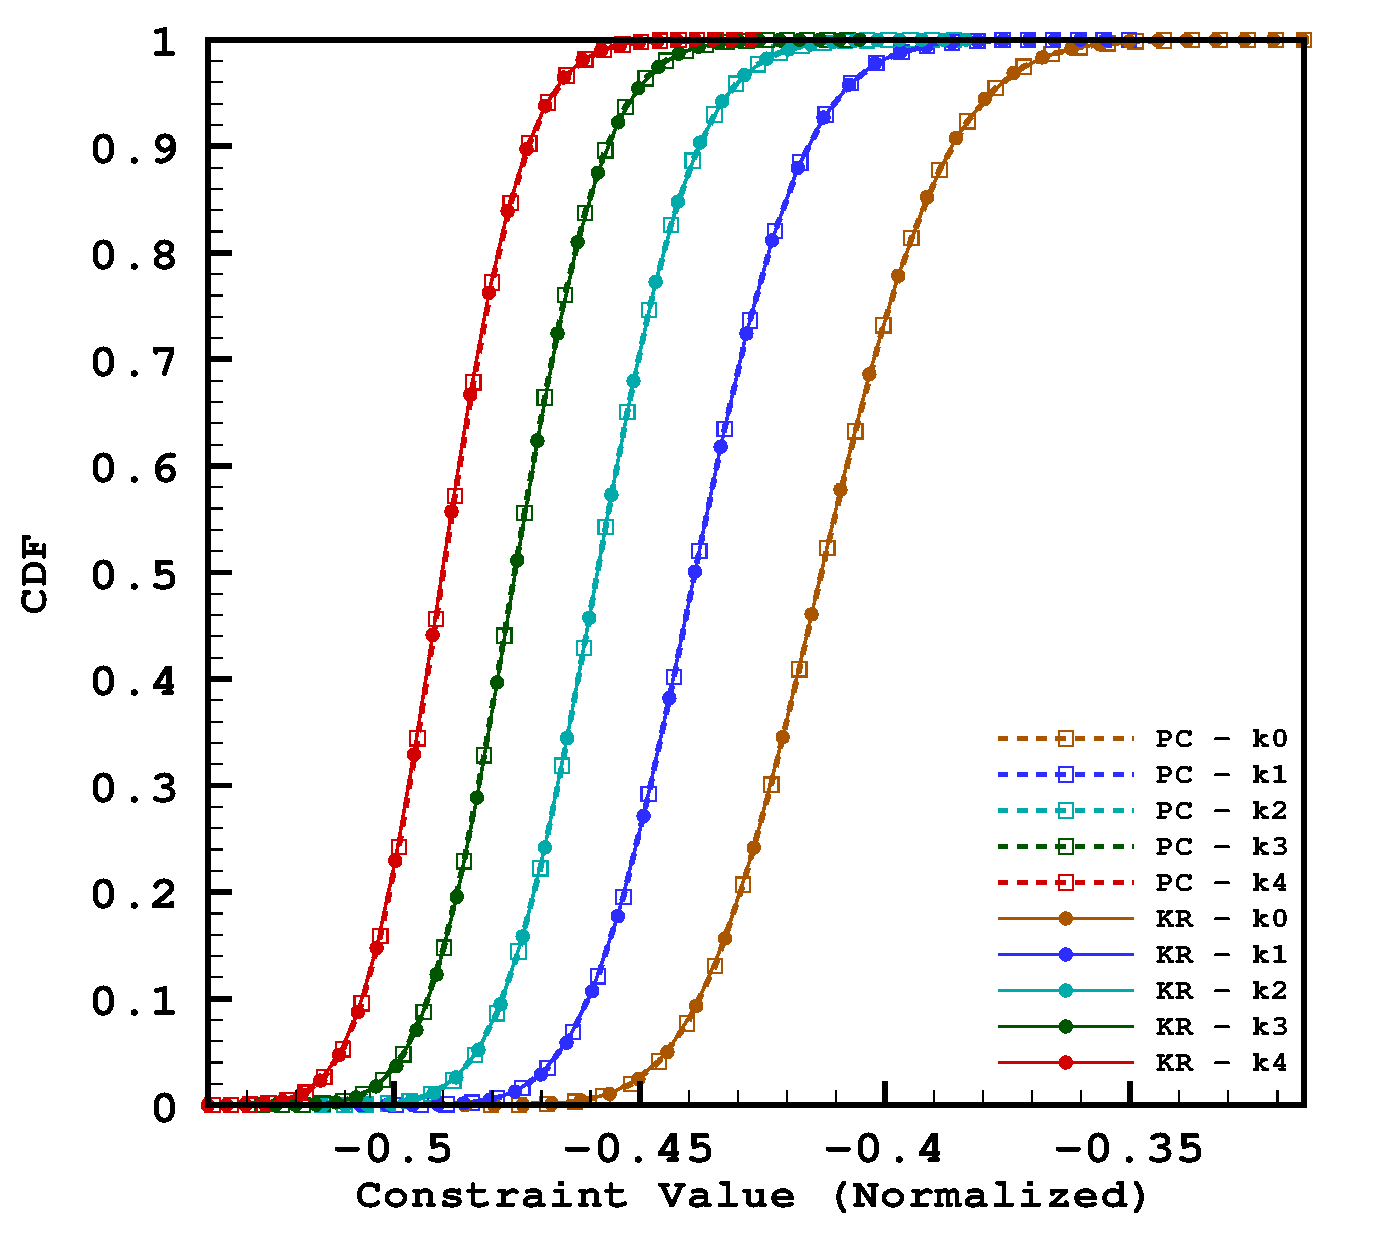
\includegraphics[width=1.0\textwidth]{3barcdfallcon2.eps} \subcaption{Constraint 2}
    \label{con2cdf}
  \end{minipage}
  \begin{minipage}[b]{0.32\linewidth}
    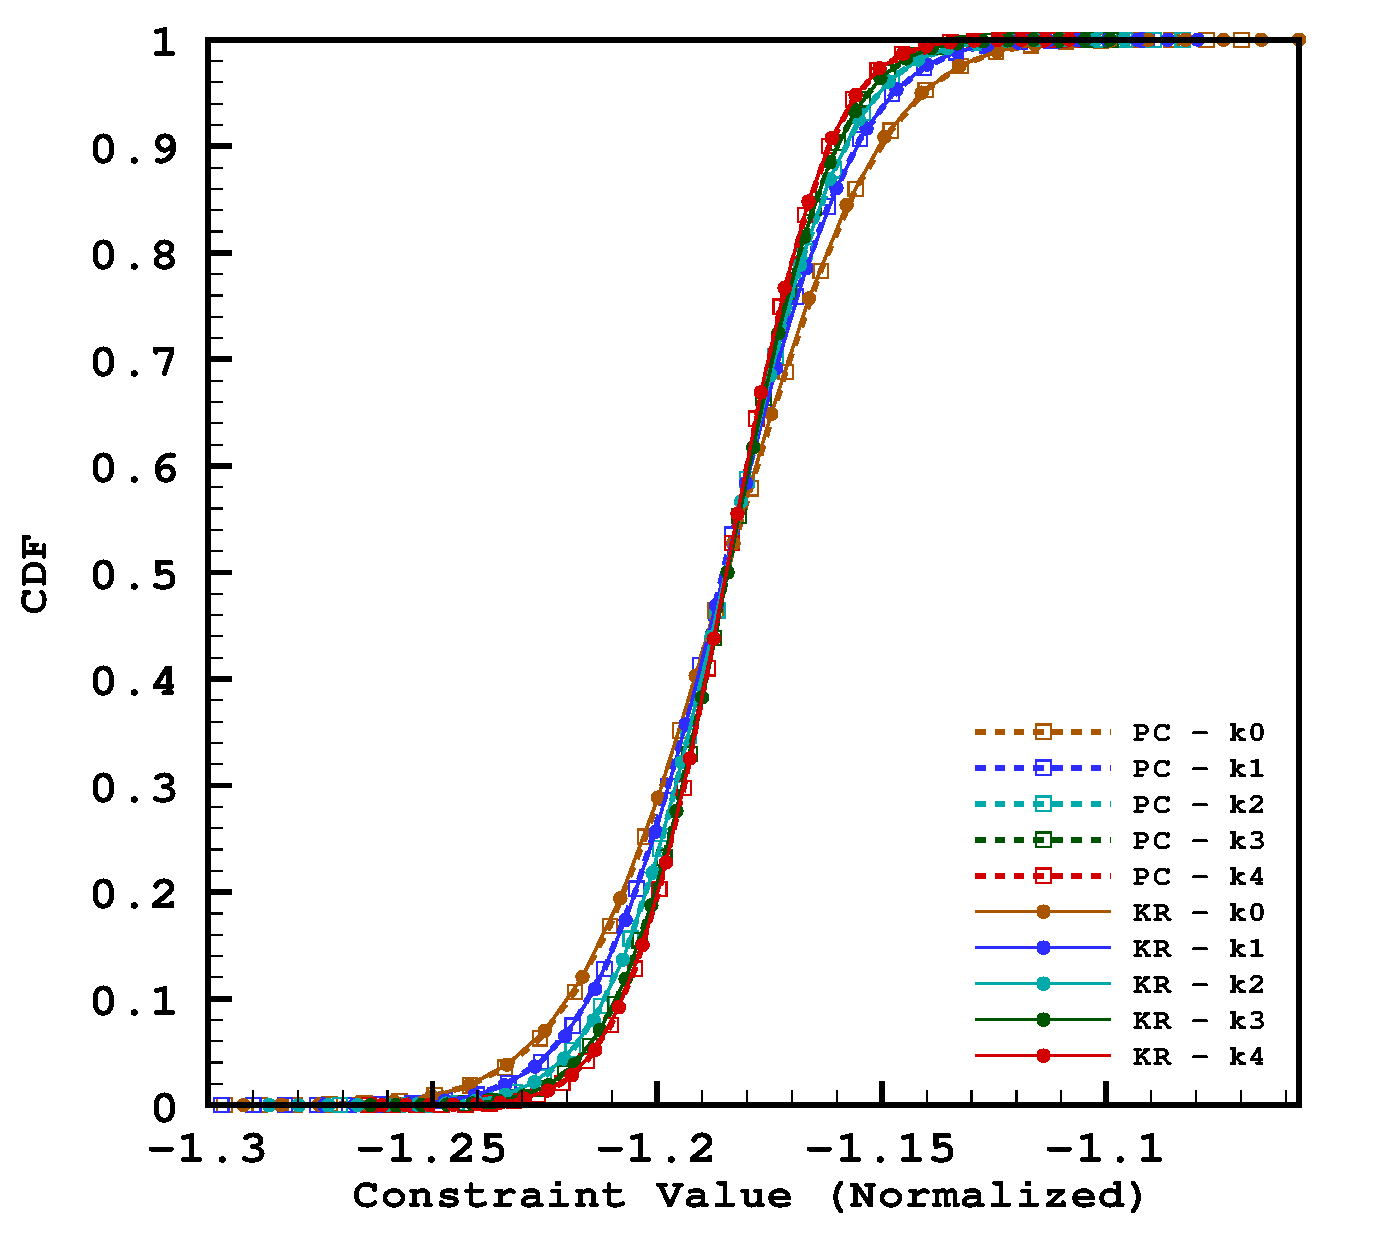
\includegraphics[width=1.0\textwidth]{3barcdfallcon3.eps} \subcaption{Constraint 3}
    \label{con3cdf}
  \end{minipage}
  \begin{minipage}[b]{0.32\linewidth}
    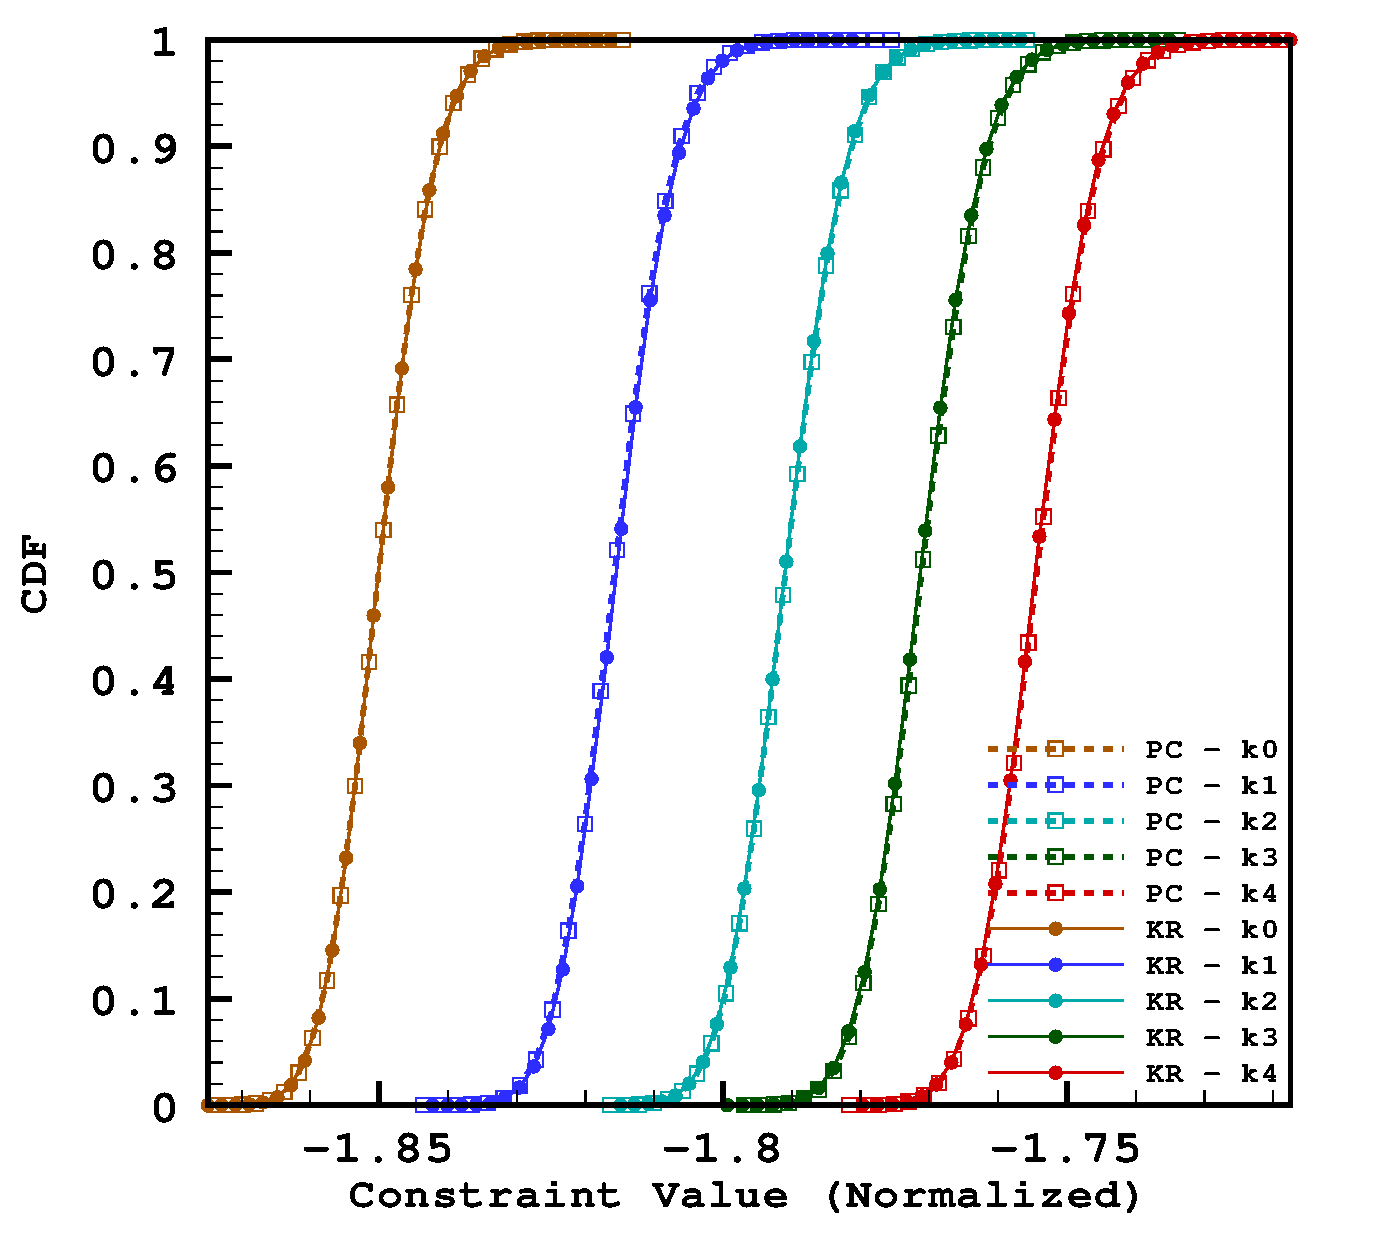
\includegraphics[width=1.0\textwidth]{3barcdfallcon4.eps} \subcaption{Constraint 4}
    \label{con4cdf}
  \end{minipage}
  \begin{minipage}[b]{0.32\linewidth}
    \includegraphics[width=1.0\textwidth]{3barcdfallcon5.eps} \subcaption{Constraint 5}
    \label{con5cdf}
  \end{minipage}
  \begin{minipage}[b]{0.32\linewidth}
    \includegraphics[width=1.0\textwidth]{3barcdfallcon6.eps} \subcaption{Constraint 6}
    \label{con6cdf}
  \end{minipage}
  \begin{minipage}[b]{0.32\linewidth}
    \includegraphics[width=1.0\textwidth]{3barcdfallcon7.eps} \subcaption{Constraint 7}
    \label{con7cdf}
  \end{minipage}
  \begin{minipage}[b]{0.32\linewidth}
    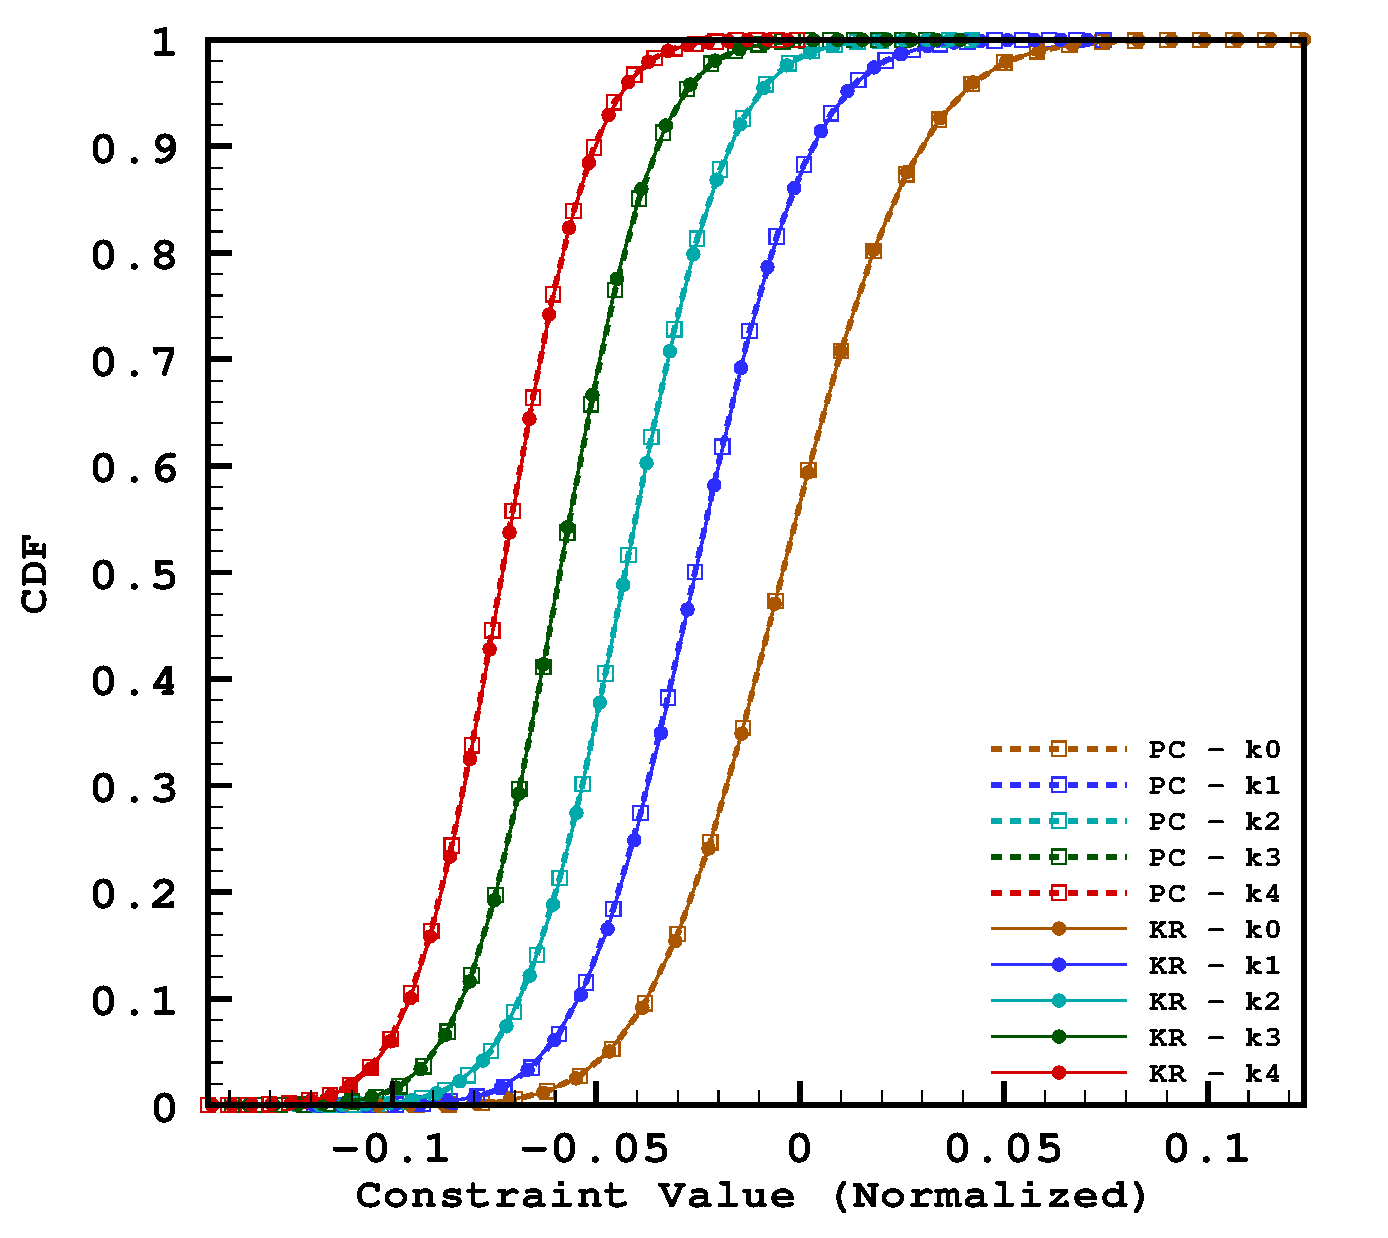
\includegraphics[width=1.0\textwidth]{3barcdfallcon8.eps} \subcaption{Constraint 8}
    \label{con8cdf}
  \end{minipage}
  \caption[Cumulative distribution functions for three-bar truss design problem.]{Cumulative distribution function of objective and constraint functions at robust optimum designs.}
  \label{3barCDF}
\end{figure}
